\section{RECONR}
\label{sRECONR}

\hypertarget{sRECONRhy}{The}
RECONR module is used to reconstruct resonance cross sections
from resonance parameters and to reconstruct cross sections from
ENDF nonlinear interpolation schemes.  The output is written as
a pointwise-ENDF (PENDF) file with all cross sections on a
unionized energy grid suitable for linear interpolation to within
a specified tolerance.  Redundant reactions (for example, total
inelastic, charged-particle reactions) are reconstructed to be
exactly equal to the sum of their reconstructed and linearized
parts at all energies.  The resonance parameters are removed from
File 2, and the material directory is corrected to reflect all
changes.  RECONR has the following features:
\index{RECONR|textbf}
\index{resonance reconstruction}
\index{resonance parameters}
\index{PENDF}
\index{union grid}
\index{redundant reactions}
\index{summation cross sections}

\begin{itemize}
\begin{singlespace}
\item  Efficient use of dynamic storage allocation and a special
       stack structure allow very large problems to be run.

\item  The unionized grid improves the accuracy, usefulness,
       and ENDF compatibility of the output.  All summation cross
       sections are preserved on the union grid.  Up to nine
       significant figures are allowed.

\item  A correct directory of the output tape is provided.

\item  Approximate $\psi\chi$ Doppler broadening
       \index{$\psi\chi$ broadening} may be used
       in some cases to speed up reconstruction.

\item  A resonance-integral criterion is added to the normal
       linearization criterion in order to reduce the number
       of points added to the tabulation to represent ``unimportant''
       resonances.

\item  All ENDF-6\index{ENDF!ENDF format!ENDF-6 format} resonance formats
       currently active are handled, including the calculation
       of angular distributions from resonance parameters in
       some cases.
\end{singlespace}
\end{itemize}

This chapter describes the RECONR module in NJOY2016.0.


\subsection{ENDF/B Cross Section Representations}
\label{ssRECONR_xsrep}

\begin{figure}[b]\centering
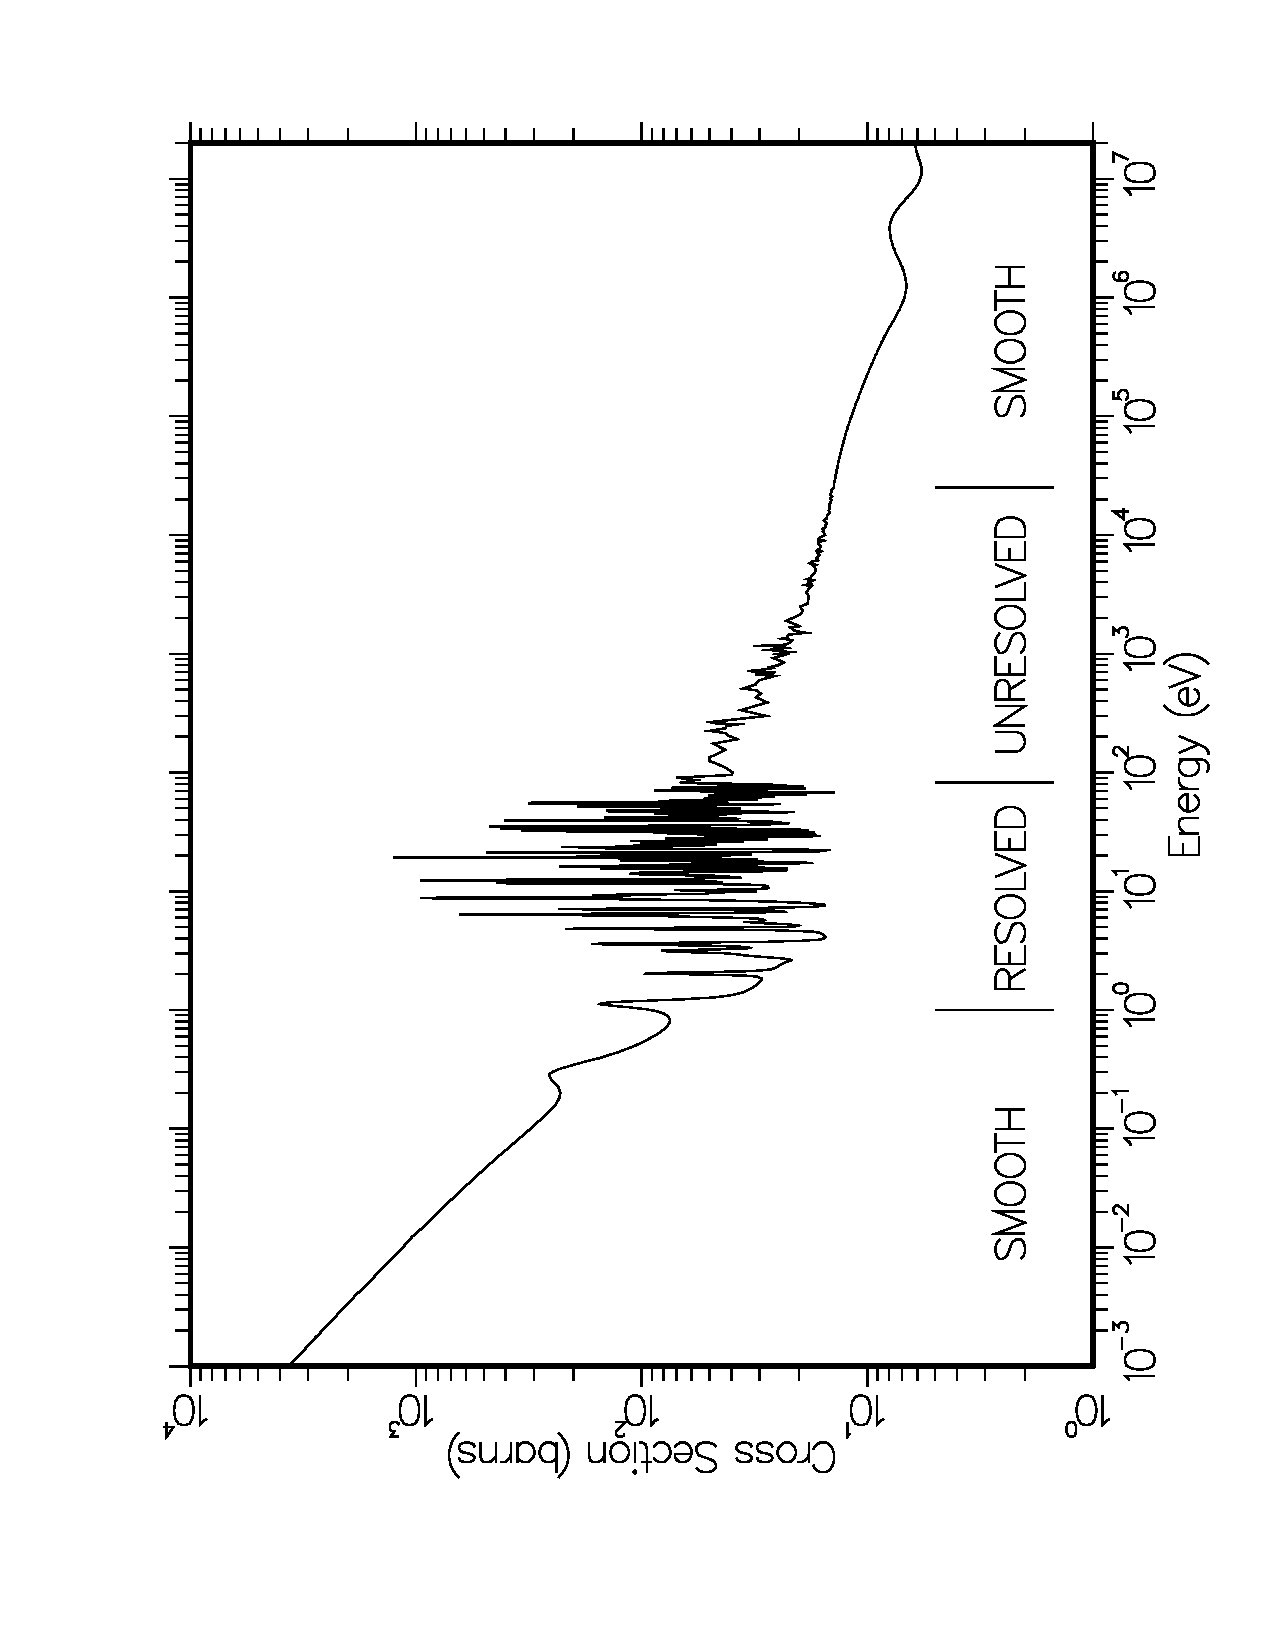
\includegraphics[keepaspectratio,height=4.0in,angle=270]{figs/reconr1ack}
\caption[RECONR reconstructed xs with smooth, RR and URR regions]{A
   typical cross section reconstructed from an ENDF/B
   evaluation using RECONR.  The smooth, resolved, and
   unresolved energy regions use different representations of the
   cross sections.  This is the total cross section for $^{235}$U
   from ENDF/B-V.}
\label{xsfig}
\end{figure}

A typical cross section derived from an ENDF/B evaluation is
shown in Fig.~\ref{xsfig}.  The low-energy cross sections are
``smooth''.\index{smooth cross sections}  They are described
in File 3 (see Section \ref{ssNJOY_ENDF_IO} for a review of
ENDF/B\index{ENDF!ENDF/B} nomenclature) using cross-section values
given on an energy grid with a specified law for
interpolation\index{interpolation} between the points.
In the resolved resonance range\index{resolved resonance range},
resonance parameters are given in File 2, and the cross sections
for resonance reactions have to be obtained by adding the
contributions of all the resonances to ``backgrounds'' from
File 3.  At still higher energies comes the unresolved
region\index{unresolved resonance range} where explicit
resonances are no longer defined.  Instead, the cross section
is computed from statistical distributions of the resonance
parameters given in File 2 and backgrounds from File 3 (or
optionally taken directly from File 3 as for smooth cross
sections).  Finally, at the highest energies, the smooth
File 3 representation is used again.

For light and medium-mass isotopes, the unresolved range is
usually omitted.  For the lightest isotopes, the resolved range
is also omitted, the resonance cross sections being given
directly in the ``smooth'' format.  In addition, several
different resonance representations are supported
(Single-Level Breit-Wigner (SLBW), Multilevel Breit-Wigner (MLBW), Adler-Adler,
Hybrid R-Function (HRF), Reich-Moore (RM), Reich-Moore-Limited (RML),
energy-independent unresolved, and energy-dependent
unresolved).  The Adler-Adler and Hybrid formats are not
being used in modern evaluations.  For an increasing number
of modern evaluations, the low energy ``smooth'' region is
omitted, and the resolved resonance region is extended to the
low energy limit.
\index{Single-Level Breit-Wigner!SLBW}
\index{Multi-Level Breit-Wigner}\index{Multi-Level Breit-Wigner!MLBW}
\index{Reich-Moore}\index{Reich-Moore!RM}
\index{Reich-Moore-Limited}\index{Reich-Moore-Limited!RML}
\index{Adler-Adler}
\index{Hybrid R-Function}\index{Hybrid R-Function!HRF}

RECONR takes these separate representations and produces a simple
cross section versus energy representation like the one shown
in Fig.~\ref{xsfig}.

\subsection{Unionization and Linearization Strategy}
\label{ssRECONR_union}

Several of the cross sections found in ENDF/B evaluations are
summation cross sections\index{summation cross sections}
(for example, total, inelastic, sometimes (n,2n) or fission,
and sometimes charged-particle reactions), and it is important
that each summation cross section be equal to the sum of its parts.
However, if the partial cross sections are represented with
nonlinear interpolation\index{interpolation!nonlinear interpolation}
\index{interpolation} schemes, the sum cannot be represented
by any simple interpolation law.  A typical case is the sum
of elastic scattering (MT=2 interpolated linearly to represent
a constant) and radiative capture (MT=102 interpolated log-log
to represent $1/v$).  The total cross section cannot be
represented accurately by either scheme unless the grid points
are very close together.  This effect leads to significant
balance errors in multigroup transport codes and to splitting
problems in continuous-energy Monte Carlo codes.\index{Monte Carlo}

The use of linear-linear interpolation ({\it i.e.,} $\sigma$ linear
in $E$)\index{interpolation!linear interpolation} can be advantageous in several
ways.  The data can be plotted easily, they can be integrated easily,
cross sections can be Doppler broadened\index{Doppler-broadening}
efficiently (see \hyperlink{sBROADRhy}{BROADR}\index{BROADR}), and,
linear data can be retrieved efficiently in continuous-energy
Monte Carlo codes. \index{Monte Carlo!continuous-energy Monte Carlo}
Therefore, RECONR puts all cross sections on a single unionized
grid suitable for linear interpolation.  As described in more
detail below, RECONR makes one pass through the ENDF/B material
to select the energy grid, and then a second pass to compute
cross sections on this grid.  Each cross section on the
PENDF\index{PENDF} file (except for the summation cross
sections\index{summation cross sections}) is exactly equal
to its ENDF/B value.  The summation cross sections are then
obtained by adding up the partial cross sections at each
grid point.

While RECONR is going through the reactions given in the ENDF/B
evaluation, it also checks the reaction thresholds\index{thresholds}
against the $Q$ value\index{Q-value} and atomic weight
ratio to the neutron $A$ (AWR\index{atomic weight ratio!AWR}
in the file) given for the reaction.  If

\begin{equation}
   {\rm threshold} \ge \frac{A+1}{A}\,Q
\end{equation}

\noindent
is not true, the threshold energy is moved up to satisfy
the condition.  This is usually a small change, often only
in the least significant digit, and is a consequence of
comparing two REAL numbers of finite precision.

If desired, the unionized grid developed from the ENDF/B file can
be supplemented with ``user grid points''\index{user grid} given
in the input data.  The code automatically adds the conventional
thermal point of 0.0253 eV and the 1, 2, and 5 points in each
decade to the grid if they are not already present.  These simple
energy grid points help when comparing materials, and they provide
well-controlled starting points for further subdivision of
the energy grid.

There are special problems with choosing the energy grid in the
unresolved range\index{unresolved resonance range}.  In some cases,
the unresolved cross section is represented using resonance
parameters that are independent of energy.  The cross sections
are not constant, however, but have a shape determined by the
energy variation of neutron wave number, penetrability factors,
and so on.  RECONR handles this case by choosing a set of energies
(about 13 per decade) to be used to calculate the cross sections;
the set of energies gives a reasonable approximation to the result
intended.  For evaluations that use energy-dependent resonance
parameters, it is supposed to be sufficient to compute the
unresolved cross sections at the given energies and to use
interpolation\index{interpolation} on the cross sections to obtain
the appropriate values at other energies.  However, some
evaluations carried over from earlier versions of ENDF/B were not
evaluated using this convention, and cross sections computed
using cross-section interpolation are not sufficiently accurate.
Even some modern evaluations use inadequate energy grids for
the unresolved range.  RECONR detects such cases by looking for
large steps between the points of the given energy grid.  It
then adds additional energy grid points using the same
13-per-decade rule used for energy-independent parameters.
``Large'' is currently defined by \cword{wide} to be a factor
of 1.26.\index{unresolved energy grid}

\subsection{Linearization and Reconstruction Methods}
\label{ssRECONR_linear}

Linearization\index{linearization} (\cword{lunion}) and resonance
reconstruction\index{resonance reconstruction} (\cword{resxs})
both function by inserting new energy grid points between
the points of an original grid using an ``inverted
stack''.\index{inverted stack}  The general concepts involved
are illustrated with a simple example shown in Fig.~\ref{stackfig}.

\begin{figure}[htbp]\centering
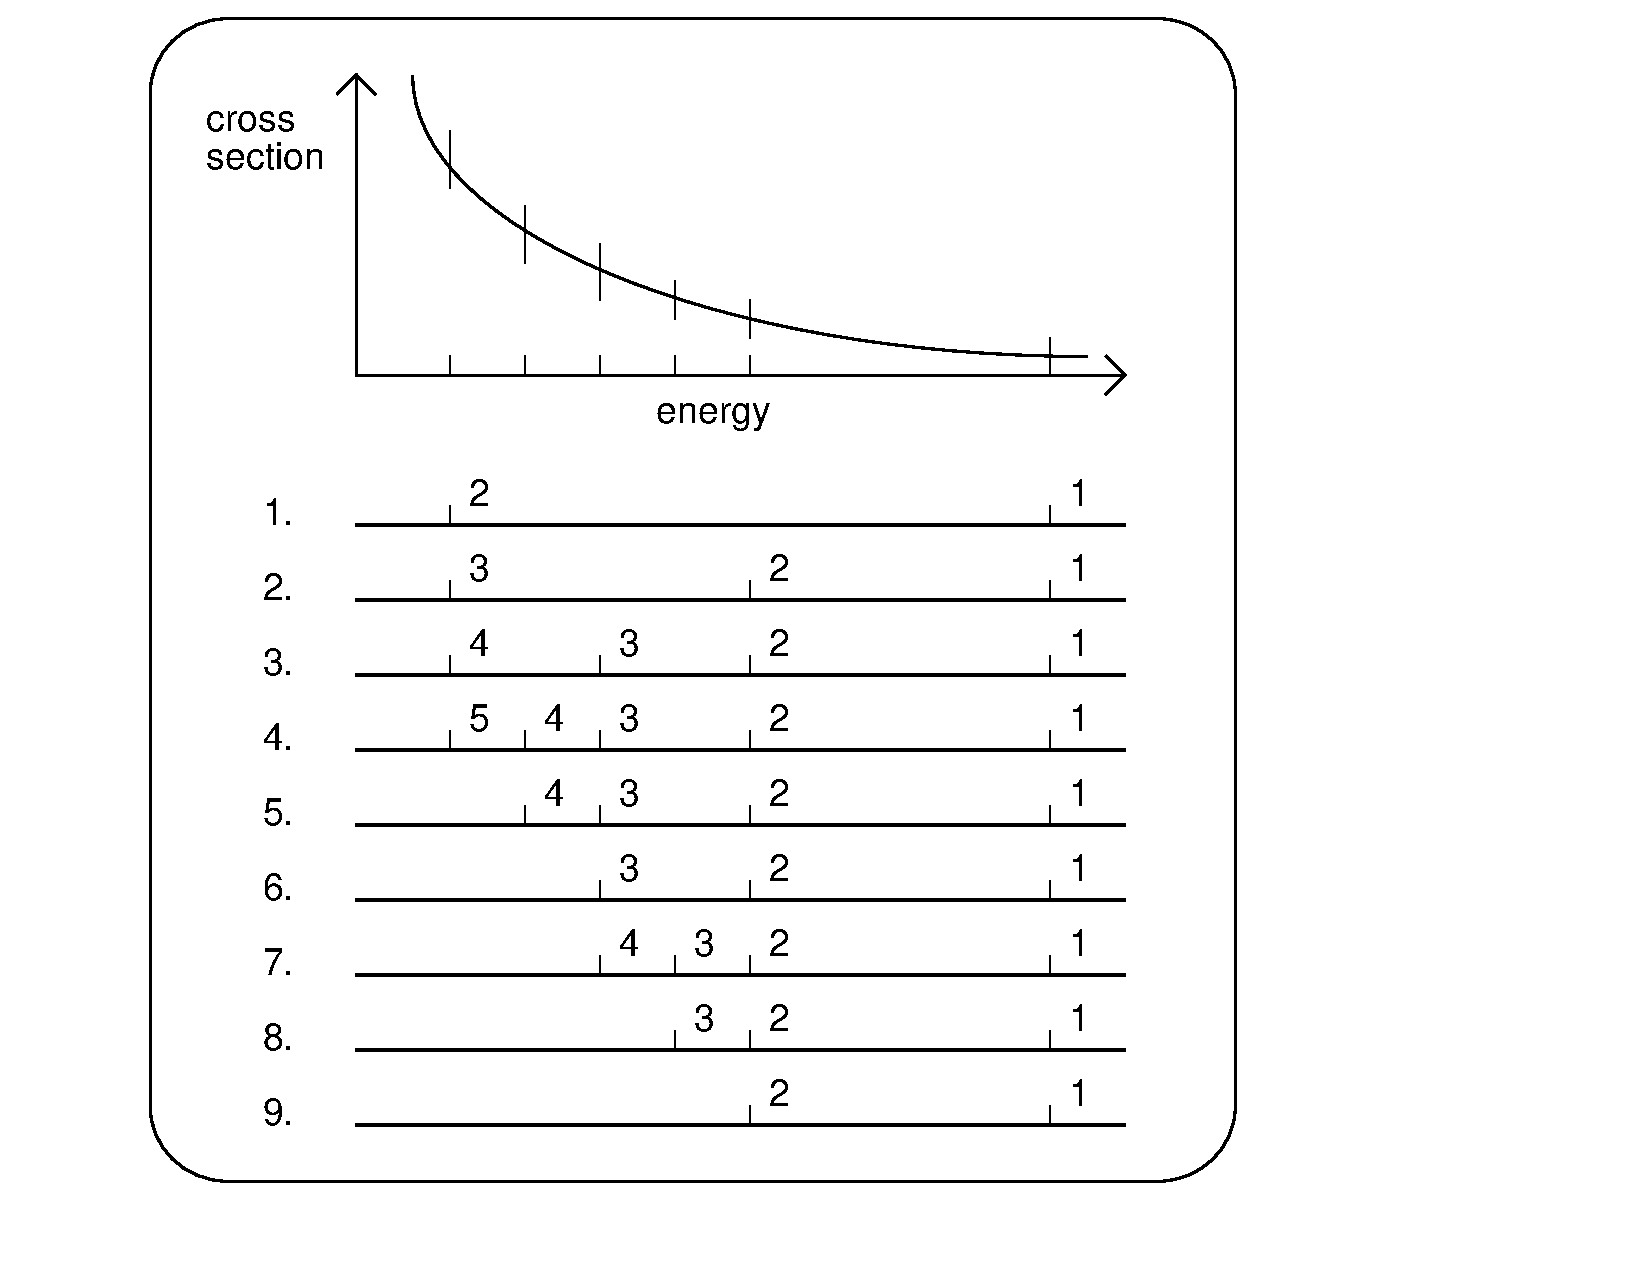
\includegraphics[keepaspectratio, height=5.3in, angle=0]{figs/reconr2ack}
\caption[Inverted stack mesh generation description]{Inverted
     -stack method used in RECONR and several
     other places in NJOY.  Line 1 shows the two initial points
     (the lower energy is higher in the stack).  In line 2, a new
     point has been calculated at the midpoint, but the result was
     not converged, and the new point has been inserted in the
     stack.  In line 3, the midpoint of the top panel has been
     checked again, found to be not converged, and inserted
     into the stack.  The same thing happens in line 4.  In line 5,
     the top panel is found to be converged, and the top point (5)
     has been written out.  The same thing happens in line 6.  In
     line 7, the top panel is tested and found to be not converged.
     The midpoint is added to the stack.  Finally, in line 8, the
     top panel is found to be converged, and the top point is
     written out.  This leaves two points in the stack (see line 9).
     Note that the energy points come off the stack in the desired
     order of increasing energy, and that only one point has to be
     moved up in the stack as each new result is inserted.}
\label{stackfig}
\end{figure}

The stack is first primed with two starting values.  For
linearization, they will be two adjacent points on the original
union grid.  For reconstruction, they will usually be the peaks
and half-height energies of resonances.  The stack is said to be
inverted because the lower energy is at the ``top''
(\cword{I}=2).

This interval or panel is now divided into two parts, and the
cross section computed at the intermediate point is compared to
the result of linear interpolation between the adjacent points.
If the two values do not agree within various criteria, the top
of the stack is moved up one notch (\cword{I}=3), and the new
value is inserted (\cword{I}=2).  The code then repeats the
checking process for the new (smaller) interval at the top of the
stack.  The top of the stack rises until convergence is achieved
for the top interval.  The top energy and cross section are then
saved on a scratch file, the stack index is decremented, and the
checks are repeated.  This process is continued with the top of
the stack rising and falling in response to the complexity of the
cross section until the entire panel $\Delta E$ has been
converged (\cword{I}=1).  The stack is then reprimed with the
bounds of the next panel.  The process continues until the entire
energy range for linearization or reconstruction has been
processed.

This stack logic enables a panel to be subdivided into parts as
small as $\Delta E / 2^n$ where $n$ is the stack size, and several
different cross sections (elastic, capture, fission) can easily
be stored in arrays of this size.

The convergence criterion used for linearization is that the
linearized cross section at the intermediate point is within the
fractional tolerance \cword{err} (or a small absolute value
\cword{errlim}) of the actual cross section specified by the
ENDF law. More complicated criteria are used for resonance
reconstruction.

There are two basic problems that arise if a simple fractional
tolerance test is used to control resonance reconstruction.
First, as points are added to the energy grid, adjacent energy
values may become so close that they will be rounded to the same
number when a formatted output file is produced.  There can be
serious problems if the code continues to add grid points after
this limit is reached.  Through the use of dynamic format
reconstruction, the energy resolution available for formatted
NJOY output (which use ENDF 11-character fields) is 7
significant figures\index{significant figures} (that is,
$\pm 1.234567\pm n$) rather than the usual 5 or 6 (see Section
\ref{ssNJOY_ENDF_IO}).  For NJOY2016, the Fortran-90 ``kind'' parameter is
used to assure sufficient precision for this.  Even this
seven significant figure format is sometimes insufficient for
very narrow resonances.  If necessary, NJOY can go to nine
significant figures by using a Fortran ``F'' format,
{\it e.g.,} $\pm 1234.56789$.

Significant-figure control is implemented as follows:  each
intermediate energy is first truncated to 7 significant
figures before the corresponding cross sections are computed.
If the resulting number is equal to either of the adjacent
values and convergence has not been obtained, subdivision
continues using energies truncated to 9 significant figures.
If an energy on this finer grid is equal to either of the
adjacent values, the interval is declared to be converged
even though convergence has not been achieved.  Thus, no
identical energies are produced, but an unpredictable but
very small loss in accuracy results.

The second basic problem alluded to above is that a very large
number of resonance grid points arise from straightforward
linear reconstruction of the resonance cross section of some
isotopes.  Many of these points come from narrow, weak,
high-energy resonances, which do not need to be treated
accurately in many applications.  As an example, the capture and
fission resonance integrals important for thermal reactors must
be computed with a $1/E$ flux weighting.  If the resonance
reconstruction tolerance is set high (say 1\%) to reduce the cost
of processing, the resonance integrals will be computed to only
1\% accuracy.  However, if the reconstruction tolerance were set
to a smaller value, like 0.1\%, and if the high-energy resonances
(whose importance is reduced by the $1/E$ weight and the $1/v$
trend of the capture and fission cross sections) were treated
with less accuracy than the low-energy resonances, then it is
likely that one could achieve an accuracy much better than 1\%
with an overall reduction in the number of points (hence computing
cost).  Since $1/E$ weighting is not realistic in all applications
(for example, in fast reactors), user control of this
``thinning'' operation must be provided.

Based on these arguments, the following approach was chosen to
control the problem of very large files.  First, panels are
subdivided until the elastic, capture, and fission cross sections
are converged to within \cword{errmax}, where \cword{errmax}
$\ge$ \cword{err}.  These two tolerances are normally chosen to
form a reasonable band, such as 1\% and 0.1\%, to ensure that
all resonances are treated at least roughly (for example, for
plotting).  If the resonance integral ($1/E$ weight) in some panel
is large, the panel is further subdivided to achieve an accuracy
of \cword{err} (say 0.1\%).  However, if the contribution to the
resonance integral from any one interval gets small, the interval
will be declared converged, and the local value of the cross
section will end up with some intermediate accuracy.  The
contribution to the error in the resonance integral should be
less than $0.5{\times}\Delta\sigma{\times}\Delta E$.  This value
is added into an accumulating estimate of the error, and a count
of panels truncated by the resonance integral check is
incremented.
\index{integral thinning}
\index{resonance integral check}

The problem with this test is that RECONR does not know the value
of the resonance integral in advance, so the tolerance parameter
\cword{errint} is not the actual allowed fractional error in the
integral.  Instead, it is more like the resonance integral error
per grid point (barns/point).  Thus, a choice of
\cword{errint=err/10000} with \cword{err}=0.001 would limit the
integral error to about 0.001 barn if 10000 points resulted from
reconstruction.  Since important resonance integrals vary from a
few barns to a few hundred barns, this is a reasonable choice.
The integral check can be suppressed by setting \cword{errint}
very small or \cword{errmax=err}.

When resonance reconstruction is complete, RECONR provides a
summary of the possible resonance integral error due to the
integral check over several coarse energy bands.  An example
from ENDF/B-VII.0 $^{235}$U follows:

\newpage
\small
\begin{ccode}

               estimated maximum error due to
               resonance integral check (errmax,errint)

    upper      elastic   percent   capture   percent   fission   percent
    energy     integral   error    integral   error    integral   error
  1.00E-05
  1.00E-04     3.50E+01   0.000    8.15E+03   0.000    4.29E+04   0.000
  1.00E-03     3.50E+01   0.000    2.57E+03   0.000    1.36E+04   0.000
  1.00E-02     3.50E+01   0.000    8.02E+02   0.000    4.24E+03   0.000
  1.00E-01     3.46E+01   0.000    2.15E+02   0.000    1.26E+03   0.000
  1.00E+00     3.25E+01   0.000    6.03E+01   0.000    3.26E+02   0.000
  2.00E+00     8.95E+00   0.000    7.31E+00   0.000    2.62E+01   0.000
  5.00E+00     1.08E+01   0.000    1.25E+01   0.000    1.56E+01   0.000
  1.00E+01     7.75E+00   0.000    2.40E+01   0.000    3.52E+01   0.000
  2.00E+01     8.18E+00   0.000    2.92E+01   0.000    3.31E+01   0.000
  5.00E+01     1.07E+01   0.000    2.57E+01   0.000    3.83E+01   0.000
  1.00E+02     8.30E+00   0.000    1.07E+01   0.000    2.34E+01   0.000
  2.00E+02     8.04E+00   0.000    8.17E+00   0.000    1.42E+01   0.000
  5.00E+02     1.10E+01   0.001    6.81E+00   0.008    1.51E+01   0.004
  1.00E+03     8.28E+00   0.008    3.44E+00   0.080    7.62E+00   0.038
  2.00E+03     8.27E+00   0.033    2.54E+00   0.261    5.06E+00   0.185

 points added by resonance reconstruction    =  232418
 points affected by resonance integral check =   80445
 final number of resonance points            =  242170
 number of points in final unionized grid    =  242600

\end{ccode}
\normalsize

\noindent
The parameters \cword{errmax} and \cword{errint}, taken together,
should be considered as adjustment ``knobs'' that can increase or
decrease the errors in the ``res-int'' columns to get an appropriate
balance between accuracy and economy for a particular application.
The error from significant figure reduction provided by earlier
versions of NJOY is no longer needed.

For energies in the thermal range (energies less than
\cword{trange}=0.5 eV), the user's reconstruction
tolerance\index{thermal reconstruction tolerance} is
divided by a factor of 5 in order to give better results for
several important thermal integrals, especially after Doppler
broadening, and to make the 0.0253 eV cross section behave
well under Doppler broadening.

\subsection{Resonance Representations}
\label{ssRECONR_resrep}

RECONR uses the resonance formulas as implemented in the original
RESEND code\cite{RESEND}\index{RESEND} with several changes:  a
more efficient calculation of MLBW cross sections \index{Multi-Level
Breit-Wigner!MLBW} developed by C. R. Lubitz\index{Lubitz} of the
Knolls Atomic Power Laboratory (KAPL)\index{Knolls Atomic Power
Laboratory!KAPL} and coded by P. Rose \index{Rose} of the National
Nuclear Data Center (NNDC)\index{National Nuclear Data Center!NNDC}
\index{NNDC|see{National Nuclear Data Center}} at
the Brookhaven National Laboratory (BNL)\index{Brookhaven National
Laboratory!BNL}, the addition of competitive widths\index{competitive width}
introduced for ENDF/B-V, a $\psi\chi$ Doppler-broadening\index{$\psi\chi$
broadening} calculation for SLBW\index{Single-Level Breit-Wigner!SLBW} and
Adler-Adler \index{Adler-Adler} resonance shapes, and a capability to
process either the multi-level multi-channel R-matrix
Reich-Moore\index{Reich-Moore!RM} parameters or
the multi-level single-channel Hybrid R-Function\index{Hybrid R-Function!HRF}
parameters based on the work of
M. Bhat\index{Bhat} and C. Dunford\index{Dunford} of the NNDC,
an implementation of the GH method\index{Multi-Level Breit-Wigner!GH MLBW
method} for MLBW resonances, which allows psi-chi broadening, and a capability
to process the new RML\index{Reich-Moore-Limited!RML}
parameters, including resolved resonance energy region angular distributions.
\index{resonance angular distributions}

Expanded discussions of the following formulas can be found in the
ENDF-6 format manual\cite{ENDF102}.\index{ENDF!ENDF format!ENDF-6 format}

\paragraph{Single-Level Breit-Wigner Representation (SLBW)}
\index{Single-Level Breit-Wigner}
The subroutine that computes Single-Level Breit-Wigner cross
sections\index{Single-Level Breit-Wigner!SLBW}
(\cword{csslbw})\index{csslbw@{\ty csslbw}} uses
\begin{eqnarray}
  \sigma_n&=&\sigma_p\nonumber\\
      & &+\sum_{\ell}\sum_r\sigma_{mr}
    \Bigl\lbrace \Bigl[ \cos 2\phi_\ell - (1-{{\Gamma_{nr}}
    \over {\Gamma_r}}) \Bigr] \,\psi(\theta,x)\nonumber\\
    & &+\sin 2\phi_\ell \,\chi(\theta,x) \Bigr\rbrace\,\,,\\
  \sigma_f&=&\sum_{\ell}\sum_r \sigma_{mr} {{\Gamma_{fr}}
     \over{\Gamma_r}}\,\psi(\theta,x)\,\,,\\
  \sigma_\gamma&=&\sum_{\ell}\sum_r\sigma_{mr} {{\Gamma_{\gamma r}}
     \over {\Gamma_r}} \,\psi(\theta,x)\,\,,\;\hbox{and}\\
  \sigma_p&=&\sum_\ell {{4\pi}\over{k^2}}(2\ell+1)\sin^2
     \theta_\ell \,\,,
\end{eqnarray}
where $\sigma_n$, $\sigma_f$, $\sigma_\gamma$, and $\sigma_p$ are
the neutron (elastic), fission, radiative capture, and potential
scattering components of the cross section arising from the given
resonances.  There can be ``background'' cross sections in File 3
that must be added to these values to account for competitive
reactions such as inelastic scattering or to correct for the
inadequacies of the single-level representation with regard to
multilevel effects or missed resonances.  The sums extend over
all the $\ell$ values and all the resolved resonances $r$ with a
particular value of $\ell$.  Each resonance is characterized by
its total, neutron, fission, and capture widths ($\Gamma,
\Gamma_n, \Gamma_f, \Gamma_\gamma$), by its $J$ value (AJ in the
file), and by its maximum value (\cword{smax}$=\sigma_{mr} /
\Gamma_r$ in the code)
\begin{equation}
   \sigma_{mr} = {\frac{4\pi}{k^2}}\,g_J \,{\frac{\Gamma_{nr}}
      {\Gamma_r}} \,\,,
\end{equation}
where $g_J$ is the spin statistical factor
\begin{equation}
   g_J={\frac{2J+1}{4I+2}}\,\,,
\end{equation}
and $I$ is the total spin (SPI) given in File 2, and $k$ is the
neutron wave number, which depends on incident energy $E$ and the
atomic weight ratio to the neutron for the isotope $A$ (AWRI in
the file), as follows:
\begin{equation}
   k=(2.196771{\times}10^{-3}){\frac{A}{A+1}}\sqrt{E}\,\,.
\end{equation}
There are two different characteristic lengths that appear in the
ENDF resonance formulas:  first, there is the ``scattering
radius''\index{scattering radius} $\hat a$, which is given
directly in File 2 as AP; and second, there is the ``channel
radius''\index{channel radius} $a$, which is given by
\begin{equation}
   a=0.123\,A^{1/3}+0.08\,\,.
\end{equation}
If the File 2 parameter NAPS is equal to one, $a$ is set equal to
$\hat a$ in calculating penetrabilities and shift factors (see
below).  The ENDF-6 option to enter an energy-dependent
scattering radius is not supported.  The neutron width in the
equations for the SLBW cross sections is energy dependent due to
the penetration factors $P_\ell$;  that is,
\index{penetrabilities}
\begin{equation}
   \Gamma_{nr}(E)={\frac{P_\ell(E)\,\Gamma_{nr}}{P_\ell(|E_r|)}}\,\,,
\end{equation}
where
\begin{eqnarray}
  P_0&=&\rho\,\,,\\
  P_1&=&{\frac{\rho^3}{1+\rho^2}}\,\,,\\
  P_2&=&{\frac{\rho^5}{9+3\rho^2+\rho^4}}\,\,,\\
  P_3&=&{\frac{\rho^7}{225+45\rho^2+6\rho^4+\rho^6}}\,\,,
              \;\hbox{and}\\
  P_4&=&{\frac{\rho^9}{11025+1575\rho^2+135\rho^4+10\rho^6+\rho^8}}\,\,,
\end{eqnarray}
where $E_r$ is the resonance energy and $\rho{=}ka$ depends on
the channel radius or the scattering radius as specified by NAPS.
The phase shifts are given by
\index{phase shifts}
\begin{eqnarray}
  \phi_0&=&\hat\rho\,\,,\\
  \phi_1&=&\hat\rho - \tan^{-1}\hat\rho \,\,,\\
  \phi_2&=&\hat\rho - \tan^{-1}{\frac{3\hat\rho}
    {3-\hat\rho^2}} \,\,,\\
  \phi_3&=&\hat\rho - \tan^{-1}{\frac{15\hat\rho-\hat\rho^3}
    {15-6\hat\rho^2}} \,\,,\;\hbox{and}\\
  \phi_4&=&\hat\rho - \tan^{-1}{\frac{105\hat\rho-10\hat\rho^3}
    {105-45\hat\rho^2+\hat\rho^4}}\,\,,
\end{eqnarray}
where $\hat\rho{=}k\hat a$ depends on the scattering radius.  The
final components of the cross section are the actual line shape
functions $\psi$ and $\chi$.  At zero temperature,
\begin{eqnarray}
  \psi&=&{\frac{1}{1+x^2}}\,\,,\\
  \chi&=&{\frac{x}{1+x^2}}\,\,,\\
  x&=&{\frac{2(E-E'_r)}{\Gamma_r}}\,\,,
\end{eqnarray}
and
\begin{equation}
   E'_r=E_r+{\frac{S_\ell(|E_r|)-S_\ell(E)}
    {2(P_\ell(|E_r|)}}\,\Gamma_{nr}(|E_r|)\,\,,
\label{r24}
\end{equation}
in terms of the shift factors
\index{resonance shift factors}
\begin{eqnarray}
  S_0&=&0\,\,,\\
  S_1&=&-{\frac{1}{1+\rho^2}}\,\,,\\
  S_2&=&-{\frac{18+3\rho^2}{9+3\rho^2+\rho^4}} \,\,,\\
  S_3&=&-{\frac{675+90\rho^2+6\rho^4}{225+45\rho^2+6\rho^4+\rho^6}}\,\,,
         \;\hbox{and}\\
  S_4&=&-{\frac{44100+4725\rho^2+270\rho^4+10\rho^6}
           {11025+1575\rho^2+135\rho^4+10\rho^6+\rho^8}}\,\,.
\end{eqnarray}
To go to higher temperatures, define
\begin{equation}
   \theta={\frac{\Gamma_r}
    {\displaystyle\sqrt{{\frac{4kTE}{A}}}}}\,\,,
\end{equation}
where $k$ is the Boltzmann constant\index{Boltzmann constant}
and $T$ is the absolute temperature.
\index{$\psi\chi$ broadening}
The line shapes $\psi$ and $\chi$ are now given by
\begin{equation}
   \psi={\frac{\sqrt{\pi}}{2}}\,\theta \,{\rm Re} W\bigl(
    {\frac{\theta x}{2}},{{\theta}\over 2}\bigr)\,\,,
\end{equation}
and
\begin{equation}
   \chi={{\sqrt{\pi}}\over 2} \,\theta \,{\rm Im}W\bigl(
    {{\theta x}\over 2},{{\theta}\over 2}\bigr)\,\,,
\end{equation}
in terms of the complex probability function (see \cword{quickw},
\cword{wtab}, and \cword{w}, which came from the MC$^2$ code\cite{MC2})
\begin{equation}
   W(x,y)={\rm e}^{-z^2}\,{\rm erfc}(-iz)
    ={\frac{i}{\pi}}\int_{-\infty}^\infty
    {{{\rm e}^{-t^2}}\over{z-t}}\,dt\,\,,
\end{equation}
where $z{=}x{+}iy$.  The $\psi\chi$ method is not as accurate as
kernel broadening\index{kernel broadening} (see
\hyperlink{sBROADRhy}{BROADR}\index{BROADR})
because the backgrounds (which are sometimes quite complex) are not
broadened, and terms important for energies less than about $16kT/A$
are neglected; however, the $\psi\chi$ method is less expensive than
\hyperlink{sBROADRhy}{BROADR}.  Previous versions of
RECONR included $\psi\chi$ broadening
\index{$\psi\chi$ broadening} for the SLBW
\index{Single-Level Breit-Wigner!SLBW} and Adler-Adler\index{Adler-Adler}
representations only.  This version also allows the method to be used
for MLBW\index{Multi-Level Breit-Wigner!MLBW} cases.  The
SLBW approach can produce negative elastic
cross sections.\index{negative cross sections} If found, they are
set to a small positive value, and a count is accumulated for a
diagnostic in the listing file.

\paragraph{Multilevel Breit-Wigner Representation (MLBW)}
\index{Multi-Level Breit-Wigner}
The Lubitz-Rose method used for calculating Multi-Level
Breit-Wigner cross sections (\cword{csmlbw}) is formulated as
follows:
\index{Lubitz-Rose method}
\index{Multi-Level Breit-Wigner!MLBW}
\index{csmlbw@{\ty csmlbw}}
\begin{equation}
  \sigma_n(E)={\frac{\pi}{k^2}}
    \sum_\ell \sum_{s=|I-\frac{1}{2}|}^{I+\frac{1}{2}}
    \sum_{J=|l-s|}^{l+s} g_J\,|1-U_{nn}^{\ell sJ}(E)|^2\,\,,
\end{equation}

\noindent with

\begin{equation}
  U_{nn}^{\ell J}(E)={\rm e}^{2i\phi_\ell}-
    \sum_r {\frac{i\Gamma_{nr}}
    {E'_r-E-i\Gamma_r/2}}\,\,,
\end{equation}

\noindent
where the other symbols are the same as those used above.
Expanding the complex operations gives

\begin{eqnarray}
  \sigma_{n}(E)&=&{\frac{\pi}{k^2}}
    \sum_\ell \sum_{s=|I-\frac{1}{2}|}^{I+\frac{1}{2}}
    \sum_{J=|l-s|}^{l+s} g_J
     \biggl\lbrace \Bigl( 1-\cos 2\phi_\ell -
    \sum_r {{\Gamma_{nr}}\over{\Gamma_r}}
    {2\over{1+x_r^2}} \Bigr)^2\nonumber\\
   &+&\Bigl(\sin 2\phi_\ell
    +\sum_r {{\Gamma_{nr}}\over{\Gamma_r}}
    {\frac{2x_r}{1+x_r^2}} \Bigr)^2 \biggr\rbrace \,\,,
\end{eqnarray}

\noindent
where the sums over $r$ are limited to resonances in spin
sequence $\ell$ that have the specified value of $s$ and $J$.
Unfortunately, the $s$ dependence of $\Gamma$ is not known.
The file contains only $\Gamma_J{=}\Gamma_{s_1J}{+}\Gamma_{s_2J}$.
It is assumed that the $\Gamma_J$ can be used for one of the
two values of $s$, and zero is used for the other.  Of course,
it is important to include both channel-spin terms in the
potential scattering.  Therefore, the equation is written in
the following form:
\index{channel spin}
\index{potential scattering}

\begin{eqnarray}
  \sigma_{n}(E)&=&{\frac{\pi}{k^2}}
    \sum_\ell \biggl[
    \sum_J g_J \biggl\lbrace \Bigl( 1-\cos 2\phi_\ell -
    \sum_r {{\Gamma_{nr}}\over{\Gamma_r}}
    {2\over{1+x_r^2}} \Bigr)^2\nonumber\\
   &+&\Bigl(\sin 2\phi_\ell
    +\sum_r {{\Gamma_{nr}}\over{\Gamma_r}}
    {\frac{2x_r}{1+x_r^2}} \Bigr)^2 \biggr\rbrace
    +2D_\ell(1-\cos 2\phi_\ell) \biggr] \,\,,
\end{eqnarray}

\noindent where the summation over $J$ now runs from

\begin{equation}
   ||I-\ell|-\frac{1}{2}| \rightarrow I+\ell+\frac{1}{2} \,\,,
\end{equation}

\noindent and $D_\ell$ gives the additional contribution to the
statistical weight resulting from duplicate $J$ values not
included in the new $J$ sum; namely,
\index{J values@{J values!duplicate $J$ values}}

\begin{eqnarray}
   D_\ell&=&
    \sum_{s=|I-\frac{1}{2}|}^{I+\frac{1}{2}}
    \sum_{J=|l-s|}^{l+s} g_J \;
    -\sum_{J=||I-\ell|-\frac{1}{2}|}^{I+\ell+\frac{1}{2}} g_J \\
    &=&(2\ell+1) \;
    -\sum_{J=||I-\ell|-\frac{1}{2}|}^{I+\ell+\frac{1}{2}} g_J\,\,.
\label{missing}
\end{eqnarray}

\noindent
A case where this correction would appear is the $\ell{=}1$ term
for a spin-1 nuclide.  There will be 5 $J$ values:  1/2, 3/2, and
5/2 for channel spin 3/2; and 1/2 and 3/2 for channel spin 1/2.
All five contribute to the potential scattering, but the file
will only include resonances for the first three.

The fission and capture cross sections are the same as for the
single-level option.  The $\psi\chi$ Doppler-broadening cannot be
used with this formulation of the MLBW representation.
\index{$\psi\chi$ broadening}\index{Multi-Level Breit-Wigner!MLBW}

However, there is an alternate representation available that
does support $\psi\chi$ broadening:
\begin{eqnarray}
  \sigma_n&=&\sigma_p\nonumber\\
      & &+\sum_{\ell}\sum_r\sigma_{mr}
    \Bigl\lbrace \Bigl[ \cos 2\phi_\ell - (1-{{\Gamma_{nr}}
    \over {\Gamma_r}})+\frac{G_{r\ell}}{\Gamma_{nr}} \Bigr]
      \,\psi(\theta,x)\nonumber\\
    & &+(\sin 2\phi_\ell +\frac{H_{r\ell}}{\Gamma_{nr}})
      \,\chi(\theta,x) \Bigr\rbrace\,\,,
\end{eqnarray}
where
\begin{equation}
   G_{r\ell}=\frac{1}{2}
    \sum_{\stackrel{\displaystyle r'\ne r}
    {\displaystyle J_{r'}\ne J_r}}
    \Gamma_{nr}\Gamma_{nr'}\frac{\Gamma_r+\Gamma_{r'}}
      {(E_r-E_{r'})^2+(\Gamma_r+\Gamma_{r'})^2/4} \,,
\end{equation}
and
\begin{equation}
   H_{r\ell}=\sum_{\stackrel{\displaystyle r'\ne r}
    {\displaystyle J_{r'}\ne J_r}}
    \Gamma_{nr}\Gamma_{nr'}\frac{E_r-E{r'}}
      {(E_r-E_{r'})^2+(\Gamma_r+\Gamma_{r'})^2/4} \,.
\end{equation}
Nominally, this method is slower than the previous one because
it contains a double sum over resonances at each energy.  However,
it turns out that G and H are slowly varying functions of energy,
and the calculation can be accelerated by computing them at just
a subset of the energies and getting intermediate values by
interpolation.  It is important to use a large number of $r'$
values on each side of $r$.  The GH MLBW method is implemented
in \cword{csmlbw2}.
\index{Multi-Level Breit-Wigner!GH MLBW method}
\index{csmlbw2@{\ty csmlbw2}}

\paragraph{Adler-Adler Representation (Adler-Adler)}
\index{Adler-Adler}
The multilevel Adler-Adler representation
 (\cword{csaa})\index{csaa@{\ty csaa}}
is defined for $\ell{=}0$ only.  It is useful for fissionable
materials.  The total cross sections are given by

\begin{eqnarray}
  \sigma_t(E)&=&{\frac{4\pi}{k^2}}\sin^2\phi_0\nonumber\\
  &+&{\frac{\pi\sqrt{E}}{k^2}} \biggl\lbrace
    \sum_r {\frac{1}{\nu_r}} \biggl[(G_r\cos 2\phi_0
    +H_r\sin 2\phi_0 ) \,\psi(\theta,x)\nonumber\\
  &+&(H_r\cos 2\phi_0 - G_r\sin 2\phi_0) \,\chi(\theta,x)
    \biggr]\nonumber\\
  &+&A_1+{\frac{A_2}{E}}+{\frac{A_3}{E^2}}
    +{\frac{A_4}{E^3}}+B_1E+B_2 E^2 \biggr\rbrace \,\,,
\end{eqnarray}

\noindent where

\begin{equation}
  x={\frac{\mu_r-E}{\nu_r}}\,\,,
\end{equation}
\vspace{0.5 pt}

\noindent and where $\nu_r$ is the resonance half-width (corresponds
to $\Gamma /2$ in the Breit-Wigner notation), $\mu_r$ is the
resonance energy, $G_r$ is the symmetric total parameter,
$H_r$ is the asymmetric total parameter, and the $A_i$ and
$B_i$ are coefficients of the total background correction.

The fission and capture cross section both use the form

\begin{eqnarray}
  \sigma_x(E)&=&{\frac{\pi\sqrt{E}}{k^2}}
    \biggl\lbrace \sum_r {\frac{1}{\nu_r}}
    \left[G_r\psi(\theta,x)+H_r\chi(\theta,x)\right]\nonumber\\
  &+&A_1+{\frac{A_2}{E}}+{\frac{A_3}{E^2}}
    +{\frac{A_4}{E^4}}+B_1E+B_2E^2 \biggr\rbrace \,\,,
\end{eqnarray}

\noindent where the values of $G$, $H$, $A_i$, and $B_i$
appropriate for the desired reaction are used.

Doppler-broadening\index{$\psi\chi$ broadening} can be applied
as for the SLBW\index{Single-Level Breit-Wigner!SLBW} case, except note
that $\Gamma_r$ in Eq.~\ref{r24} must be replaced with $2\nu_r$.
Doppler-broadened Adler-Adler cross sections are more accurate
than SLBW cross sections because the background is smoother.
However, cross sections below about $16kT/A$ will still be
inaccurate.  The Adler-Adler method is not used in modern
evaluations.

\paragraph{Reich-Moore Representation (RM)}\index{Reich-Moore}
The Reich-Moore representation\index{Reich-Moore!RM}
as implemented in subroutine \cword{csrmat}\index{csrmat@{\ty csrmat}}
is a multi-level formulation with two fission channels; hence,
it is useful for both structural and fissionable materials.
The cross sections are given by

\begin{eqnarray}
    \sigma_t&=&{\frac{2\pi}{k^2}}\sum_\ell\sum_J
        g_J \Bigl\{ \bigl( 1-{\rm Re}\,U_{nm}^{\ell J}
        \bigr) + 2d_{\ell J}\bigl[1-\cos(2\phi_\ell)
        \bigr]\Bigr\} \,\,,\\
    \sigma_n&=&{\frac{\pi}{k^2}}\sum_\ell\sum_J
      g_J \Bigl\{ | 1-U_{nn}^{\ell J} |^2
         + 2d_{\ell J}\bigl[1-\cos(2\phi_\ell) \Bigr]
        \,\,,\\
    \sigma_f&=&{\frac{4\pi}{k^2}}\sum_\ell\sum_J
      g_J \sum_c |{\cal I}_{nc}^{\ell J} |^2 \,\,,\;\hbox{and}\\
  \sigma_\gamma&=&\sigma_t-\sigma_n-\sigma_f \,\,,
\end{eqnarray}

\noindent where ${\cal I}_{nc}$ is an element of the inverse of the
complex R-matrix\index{R-matrix} and

\begin{equation}
  U_{nn}^{\ell J}={\rm e}^{2i\phi_\ell}\,
    \Bigl[ \,2{\cal I}_{nn}-1\, \Bigr] \,\,.
\label{ufun}
\end{equation}

\noindent The elements of the R-matrix are given by

\begin{equation}
  R_{nc}^{\ell J}=\delta_{nc}
    -{\frac{i}{2}}\sum_r {{\Gamma_{nr}^{1/2}\Gamma_{cr}^{1/2}}
    \over{E_r-E-{\frac{i}{2}}\Gamma_{\gamma r}}}\,\,.
\end{equation}
\vspace{0.5 pt}

\noindent In these equations, ``c'' stands for the fission channel, ``r''
indexes the resonances belonging to spin sequence ($\ell,J$), and
the other symbols have the same meanings as for SLBW or MLBW.  Of
course, when fission is not present, $\sigma_f$ can be ignored.
The R-matrix reduces to an R-function\index{R-function}, and
the matrix inversion normally required to get ${\cal I}_{nn}$
reduces to a simple inversion of a complex number.

As in the MLBW\index{Multi-Level Breit-Wigner!MLBW} case, the
summation over $J$ runs from

\begin{equation}
   ||I-\ell|-\frac{1}{2}| \rightarrow I+\ell+\frac{1}{2} \,\,.
\end{equation}

\noindent The term $d_{\ell J}$ in the expressions for the total and
elastic cross sections is used to account for the possibility
of an additional contribution to the potential scattering
cross section from the second channel spin.  It is unity
if there is a second $J$ value equal to $J$, and zero otherwise.
This is just a slightly different approach for making the
correction discussed in connection with Eq.~(\ref{missing}).
Returning to the $I{=}1$, $\ell{=}1$ example given above,
$d$ will be one for $J{=}1/2$ and $J{=}3/2$, and it will
be zero for $J{=}5/2$.

ENDF-6 format RM evaluations can contain a parameter
LAD that indicates that these parameters can be used to compute an
angular distribution\index{resonance angular distributions}
for elastic scattering if desired (an approximate angular
distribution is still given in File 4 for these cases).  The
current version of RECONR has such a capability, and it can
be used with RM\index{Reich-Moore!RM} evaluations.  Because of channel-spin
issues, it works best with RML\index{Reich-Moore-Limited!RML} evaluations.
See below for a discusion of angular distributions.

\paragraph{Hybrid R-Function Representation (HRF)}\index{Hybrid R-Function}
The Hybrid R-Function representation\index{Hybrid R-Function!HRF} treats
elastic scattering as a multi-level
cross section using formulas similar to those given above
for the Reich-Moore\index{Reich-Moore!RM} format
in the case where fission is absent.  The other reactions are
treated with formulas similar to those of the SLBW\index{Single-Level
Breit-Wigner!SLBW} method.  The main use for this format is to provide a better
representation of competitive reactions than is
provided by any of the other formats described above.  This
treatment can include a background R-function, tabulated
charged-particle penetrabilities, and optical model phase
shifts.  Following the RM notation, the elastic cross
section is given by
\begin{equation}
    \sigma_n={\frac{\pi}{k^2}}
    \sum_\ell \sum_{s=|I-\frac{1}{2}|}^{I+\frac{1}{2}}
    \sum_{J=|l-s|}^{l+s}
      g_J | 1-U_{nn}^{\ell sJ} |^2\,\,,\\
\end{equation}
where the $U$ function is given by the scalar version of
Eq.~(\ref{ufun}):
\begin{equation}
  U_{nn}^{\ell sJ}={\rm e}^{2i\phi_\ell}\,
    \Bigl[\,\frac{2}{R^{\ell sJ}_{nn}}-1\, \Bigr] \,\,.
\end{equation}
The R-function\index{R-function} itself is given by
\begin{equation}
  R_{nn}^{\ell sJ}=1
    -{\frac{i}{2}}\sum_r {{\Gamma_{nr}}\over
    {E_r-E-{\frac{i}{2}}\Gamma_{\gamma r}}}
     -i\,P_{\ell sJ}R^0_{\ell sJ}\,\,,
\end{equation}
where $R^0_{\ell sJ}$ is a (complex) background R function and
$P_{\ell sJ}$ is a penetrability factor.  The background R
function can either be read in or set to zero.  The penetrability
and shift factors are computed from the scattering radius or
channel radius as for SLBW\index{Single-Level Breit-Wigner!SLBW}.  The phase
shifts $\phi_{\ell sJ}$ can be computed from the scattering radius
as before, or the (complex) phase shifts can be read in from
an optical model calculation.

Note that resonance parameters are given explicitly for all three
quantum numbers $\ell$, $s$, and $J$.  No correction to the
potential scattering cross section from repeated $J$ values is
needed.

Elastic angular distributions can also be computed from HRF
parameters if the LAD parameter is set;  however, RECONR does not
support that.

\paragraph{Reich-Moore-Limited Representaton (RML)}
\index{Reich-Moore-Limited}  The Reich-Moore-Limited representation is a more
general multilevel and multichannel formulation. In addition to the
normal elastic, fission, and capture reactions, it allows for
inelastic scattering and Coulomb reactions.  Furthermore,
it allows resonance angular distributions to be calculated.
It is also capable of computing derivatives of cross sections
with respect to resonance parameters.  See
\hyperlink{sERRORRhy}{ERRORR}.  The RML
processing in NJOY is based on the SAMMY code\cite{SAMMY}.
The calculation in RECONR makes use of several subroutines
exported by the \cword{samm} module;\index{modules!samm@{\ty samm}}
namely, \cword{s2sammy}, \cword{ppsammy}, \cword{rdsammy},
\cword{cssammy}, and \cword{desammy}.
\index{Reich-Moore-Limited!RML}
\index{SAMMY}
\index{ppsammy@{\ty ppsammy}}
\index{rdsammy@{\ty rdsammy}}
\index{cssammy@{\ty cssammy}}
\index{s2sammy@{\ty s2sammy}}
\index{desammy@{\ty desammy}}

The quantities that are conserved during neutron scattering and
reactions are the total angular momentum $J$ and its associated
parity $\pi$, and the RML format lumps all the channels with
a given $J^\pi$ into a ``spin group.''\index{spin group} In
each spin group, the reaction channels are defined by
$c=(\alpha,\ell,s,J)$, where $\alpha$ stands for the
particle pair (masses, charges, spins, parities, and Q-value),
$\ell$ is the orbital angular momentum with associated
parity $(-1)^\ell$, and $s$ is the channel spin (the
vector sum of the spins of the two particles of the pair).  The
$\ell$ and $s$ values must vector sum to $J^\pi$ for the spin group.
The channels are divided into incident channels and exit
channels.  Here, the important input channel is defined by the
particle pair neutron+target.  There can be several such
incident channels in a given spin group.  The exit channel
particle pair defines the reaction taking place.  If the
exit channel is the same as the incident channel, the reaction
is elastic scattering.  There can be several exit channels
that contribute to a given reaction.

The R-matrix\index{R-matrix} in the Reich-Moore ``eliminated width''
\index{eliminated width} approximation for a given spin group is
given by
\begin{equation}
  R_{cc'}=\sum_\lambda \frac{\gamma_{\lambda c}\gamma_{\lambda c'}}
     {E_\lambda-E-i\Gamma_{\lambda\gamma}/2}
     +R_c^b\delta_{cc'}\,,
\label{rmtx}
\end{equation}
where $c$ and $c'$ are incident and exit channel indexes, $\lambda$
is the resonance index for resonances in this spin group,
$E_\lambda$ is a resonance energy, $\gamma_{\lambda c}$ is a
resonance amplitude, and $\Gamma_{\lambda\gamma}$ is the
``eliminated width,'' which normally includes all of the
radiation width (capture).  The channel indexes runs over the
``particle channels'' only, which doesn't include capture.
The quantity $R_c^b$ is the ``background R-matrix.''
\index{background R-matrix}

In order to calculate the contribution of this spin group to the
cross sections, we first compute the following quantity:
\begin{equation}
  X_{cc'}=P_c^{1/2}\,L_c^{-1} \sum_{c''} Y_{cc''}^{-1}
      R_{c''c'}\,P_{c'}^{1/2} \,,
\label{xmtx}
\end{equation}
where
\begin{equation}
  Y_{cc''}=L_c^{-1}\delta_{cc''}-R_{cc''} \,,
\end{equation}
and
\begin{equation}
  L_c=S_c-B_c+iP_c \,.
\end{equation}
Here, the $P_c$ and $S_c$ are penetrability\index{penetrability
factor} and shift factors,\index{shift factor} and the $B_c$ are
boundary constants.  The cross sections can now be written down
in terms of the $X_{cc'}$.  For elastic scattering
\begin{equation}
  \sigma_{elastic}=\frac{4\pi}{k_\alpha^2}\sum_{J^\pi}
  \Bigl[\sin^2\phi_c(1-2X_{cc}^i) \nonumber\\
   -X_{cc}^r\sin(2\phi_c)
    +\sum_{c'}|X_{cc'}|^2\Bigr] \,,
\end{equation}
where $X_{cc'}^r$ is the real part of $X_{cc'}$, $X_{cc'}^i$ is
the imaginary part, $\phi_c$ is the phase shift, the sum over
\index{phase shifts}
$J^\pi$ is a sum over spin groups, the sum over $c$ is limited to
incident channels in the spin group with particle pair $\alpha$
equal to neutron+target, and the sum over $c'$ is limited to
exit channels in the spin group with particle pair $\alpha$.
Similarly, the capture cross section becomes
\begin{equation}
  \sigma_{capture}=\frac{4\pi}{k_\alpha^2}\sum_{J^\pi}
     \sum_c g_{J\alpha}\sum_c\Bigl[X_{cc}^i
   -\sum_{c'}|X_{cc'}|^2\Bigr] \,,
\end{equation}
where the sum over $J^\pi$ is a sum over spin groups, the sum over
$c$ is a sum over incident channels in the spin group with
particle pair $\alpha$ equal to neutron+target, and the sum
over $c'$ includes all channels in the spin group.  The cross
sections for other reactions (if present) are given by
\begin{equation}
  \sigma_{reaction}=\frac{4\pi}{k_\alpha^2}\sum_{J^\pi}
   g_{J\alpha}\sum_c\Bigl[X_{cc}^i-\sum_{c'} |X_{cc'}|^2\Bigr] \,,
\end{equation}
where the sum over $c$ is limited to channels in the spin group
$J^\pi$ with particle pair $\alpha$ equal to neutron+target, and
the sum over $c'$ is limited to channels in the spin group with
particle pair $\alpha'$.  The reaction is defined by
$\alpha\rightarrow\alpha'$.  This is one of the strengths
of the RML representation.  The reaction cross sections can
include multiple inelastic levels with full resonance behavior.
They can also include cross sections for outgoing charged particles,
such as (n,$\alpha$) cross sections, with full resonance
behavior.  The total cross section can be computed by summing
up its parts.

For non-Coulomb channels, the penetrabilities $P$, shift factors
$S$, and phase shift $\phi$ are the same as those given for
the SLBW representation, except if a Q value is present, $\rho$
must be modified as follows:
\begin{equation}
   \rho=(2.196771{\times}10^{-3}){\frac{A}{A+1}}
     \sqrt{|E+\frac{A+1}{A}Q|}\,\,.
\end{equation}
These factors are a little more complicated for Coulomb channels.
See the SAMMY reference for more details.\index{Coulomb channels}

The RML\index{Reich-Moore-Limited!RML} representation is new to the ENDF
format, and it isn't represented by any cases in ENDF/B-VII.0.  There are
experimental evaluations for $^{19}$F and $^{35}$Cl from ORNL\index{Oak Ridge
National Laboratory!ORNL} available.  However, the RML approach provides
a very faithful representation of resonance physics, and it should see
increasing use in the future.

\paragraph{RML Angular Distributions.} One of the physics
advances available when using the RML format is the calculation
of angular distributions from the resonance parameters.
\index{angular distributions}\index{Reich-Moore-Limited!RML}
A Legendre representation is used:
\begin{equation}
  \frac{d\sigma_{\alpha\alpha'}}{d\Omega_{\rm CM}}
     =\sum_L B_{L\alpha\alpha'}(E)P_L(\cos\beta) \,,
\end{equation}
where the subscript $\alpha\alpha'$ indicates the cross section
as defined by the two particle pairs, $P_L$ is the Legendre
polynomial of order $L$, and $\beta$ is the angle of the outgoing
particle with respect to the incoming neutron in the CM system.
The coefficients $B_{L\alpha\alpha'}(E)$ are given by a
complicated six level summation over the elements of the
scattering matrix $U$, where
\begin{equation}
   U_{cc'}=\Omega_c W_{cc'} \Omega_{c'} \,,
\end{equation}
where
\begin{equation}
  \Omega_c={\rm e}^{i(w_c-\phi_c)} \,,
\end{equation}
and
\begin{equation}
   W=I+2iX \,,
\end{equation}
with $I$ being the identity matrix and $X$ having been
already given in Eq.~\ref{xmtx}.  The coefficients $B$
become
\begin{eqnarray}
   B_{L\alpha\alpha'}(E)&=&\frac{1}{4k_\alpha^2}
     \sum_A \sum_B \sum_C \sum_D \sum_E \sum_F
    \frac{1}{(2i+1)(2I+1)} \nonumber\\
  &\times& G_{c_1c'_1;c_2c'_2;L}\, {\rm Re}[(\delta_{c1c'_1}
    -U_{c_1c'_1})(\delta_{c_2c'_2}-U^*_{c_2c'_2})] \,.
\end{eqnarray}
The spins $I$ and $i$ are for the target and projectile
for particle pair $\alpha$.  The complex expressions for the
geometric coefficient $G$ are given in the SAMMY documentation.
The six summations are as follows:

\begin{tabular}{ll}
    &                                                              \\
 A & sum over spin groups defined by $J^\pi_1$ \\
 B & sum over spin groups defined by $J^\pi_2$ \\
 C & sum over entrance channels $c_1$ belonging
    to group $J^\pi_1$ with particle pair $\alpha$ \\
 D & sum over exit channels $c'_1$ belonging
    to group $J^\pi_1$ with particle pair $\alpha'$ \\
 E & sum over entrance channels $c_2$ belonging
    to group $J^\pi_2$ with particle pair $\alpha$ \\
 F & sum over exit channels $c'_2$ belonging
    to group $J^\pi_2$ with particle pair $\alpha'$ \\
    &                                                              \\
\end{tabular}

\noindent Fig.~\ref{adist} shows the first few Legendre
coefficients for the elastic scattering cross sections as
computed by NJOY from the experimental evaluation for $^{19}$F.

\begin{figure}[ht]\centering
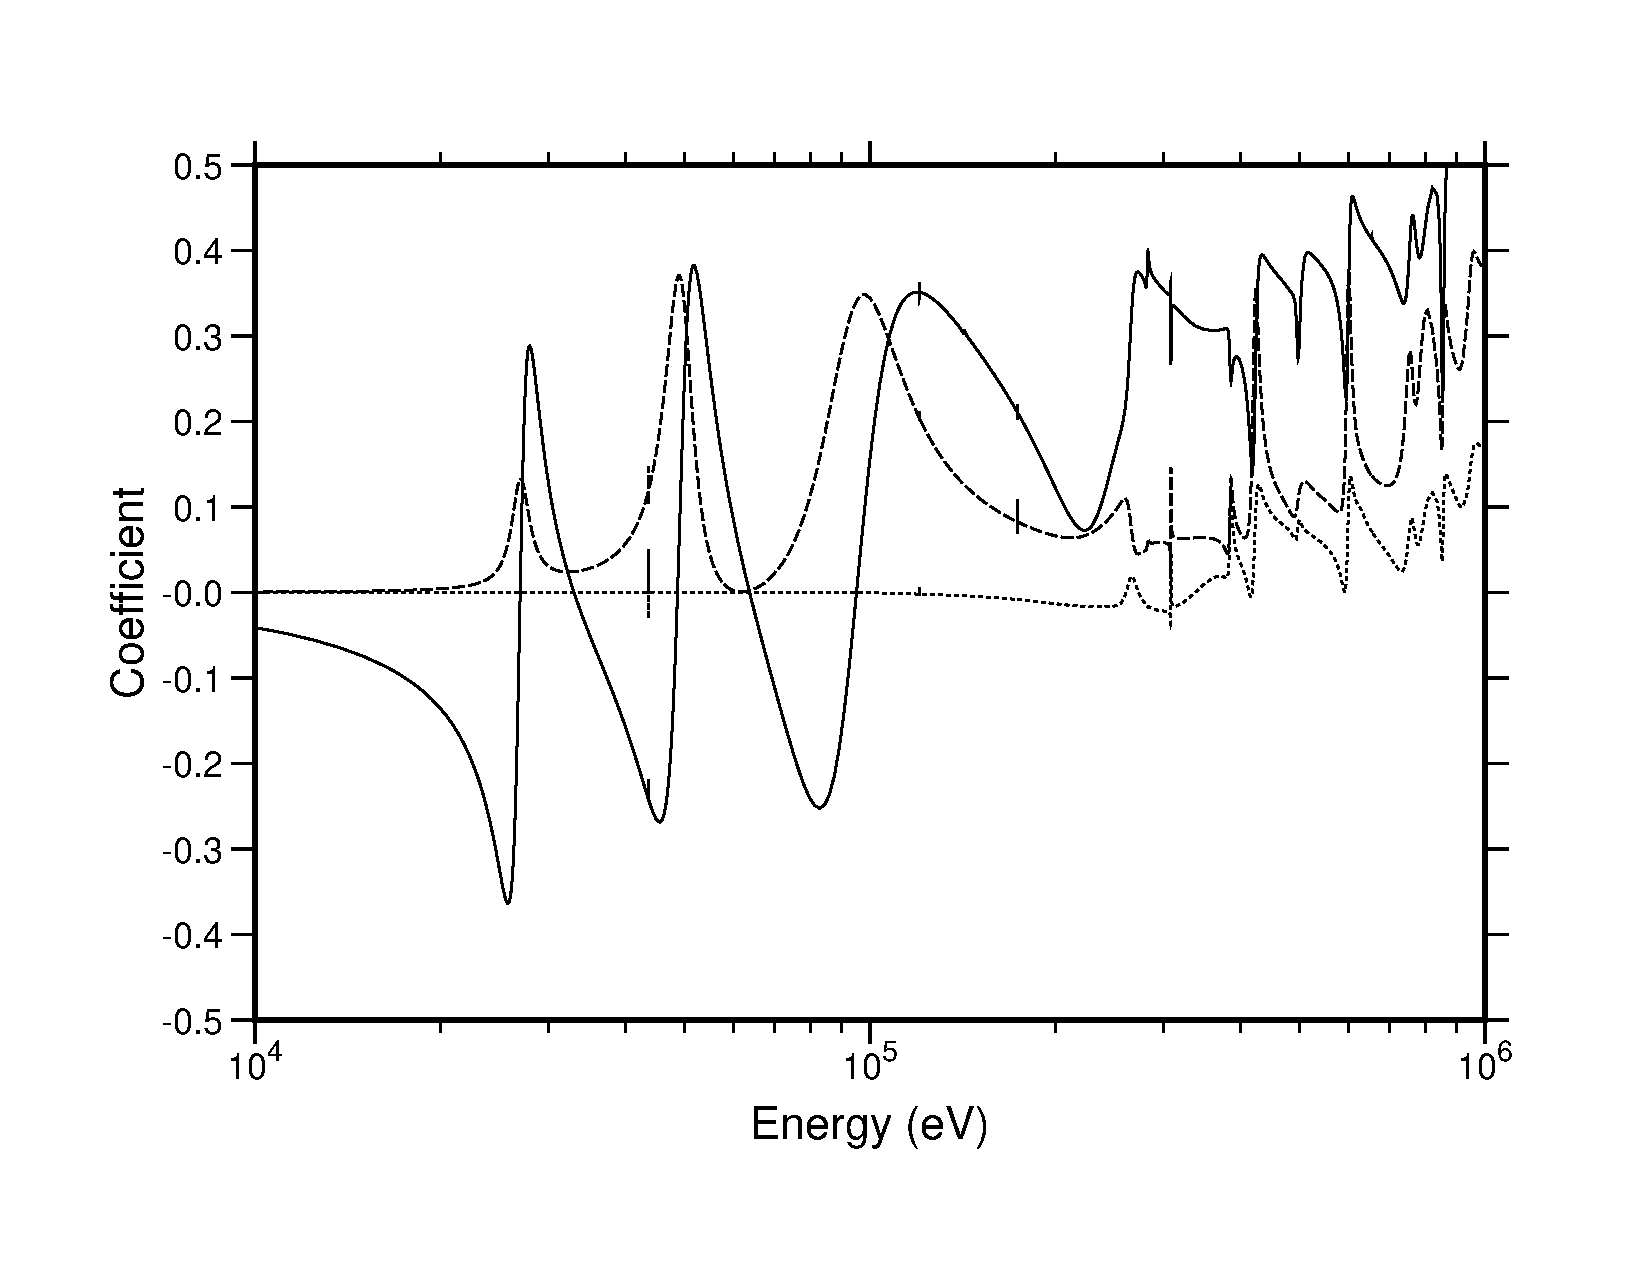
\includegraphics[height=3.5in, angle=0]{figs/adist_ack}
\caption[$^{19}$F elastic scattering Legendre coefficients from RML data]
  {Legendre coefficients of the angular distribution for
   elastic scattering in $^{19}$F using the RML resonance
   representation (P$_1$ solid, P$_2$ dashed, P$_3$ dotted).}
\label{adist}
\end{figure}

Although first introduced in NJOY2012, computing resonance
angular distributions is a new, little used feature, and so
it is not enabled by default.  To activate it, change
\cword{Want\_Angular\_Dist}\index{Want\_Angular\_Dist@{\ty Want\_Angular\_Dist}}
to true.  The Legendre coefficients are written into a section of
File 4 on the RECONR PENDF\index{PENDF} file.  Because the normal
ENDF File 4 sections are not copied to the PENDF File 4, the
presence of File 4 on a PENDF file can be detected by subsequent modules,
such a \hyperlink{sACERhy}{ACER}\index{ACER} or
\hyperlink{sGROUPRhy}{GROUPR}\index{GROUPR}, and the resonance
angular distributions can be used to replace the ENDF File 4 values
over the resonance energy range.  The default in NJOY2016 is to use
the conventional RM\index{Reich-Moore!RM} processing path for RM parameters.
However, there is an option to convert the RM parameters
into RML\index{Reich-Moore-Limited!RML} format and process them with the
RML methods.  If this is done, resonance angular distributions can be
computed for an RM evaluation.  Change \cword{Want\_SAMRML\_RM}
\index{Want\_SAMRML\_RM@{\ty Want\_SAMRML\_RM}} to true.

\paragraph{Infinitely-Dilute Unresolved Range Parameters}
Infinitely dilute cross sections in the unresolved-energy range
\index{unresolved resonance range} are computed in
\cword{csunr1}\index{csunr1@{\ty csunr1}} or
\cword{csunr2}\index{csunr2@{\ty csunr2}} using average
resonance parameters and probability distributions from File 2.
With the approximations used, these cross sections are not
temperature dependent; therefore, the results are a good match to
resolved resonance data generated using \cword{tempr}$>$0.  The
formulas used are based on the SLBW\index{Single-Level Breit-Wigner!SLBW}
approximation with interference.
\begin{eqnarray}
  \sigma_n (E) &=& \sigma_p
    +{\frac{2\pi^2}{k^2}} \sum_{\ell,J}
    {\frac{g_J}{\overline D}} \bigl[
    \overline\Gamma_n^2 R_n
    -2\overline\Gamma_n\sin^2\phi_\ell \bigr]
    \,\,,\\
  \sigma_x(E)&=&{\frac{2\pi^2}{k^2}}
    \sum_{\ell,J} {\frac{g_J}{\overline D}}
    \,\overline\Gamma_n \overline\Gamma_x R_x
    \,\,,\;\hbox{and}\\
  \sigma_p&=&{\frac{4\pi}{k^2}} \sum_\ell
    (2\ell+1)\sin^2\phi_\ell
    \,\,,
\end{eqnarray}
where $x$ stands for either fission or capture, $\overline
\Gamma_i$ and $\overline D$ are the appropriate average widths
and spacing for the $\ell{,}J$ spin sequence, and $R_i$ is the
fluctuation integral for the reaction and sequence (see
\cword{gnrl}).  These integrals are simply the averages taken
over the chi-square distributions\index{chi-square distributions}
specified in the file; for example,
\begin{eqnarray}
  \overline\Gamma_n\overline\Gamma_f R_i&=&
    \biggl< {\frac{\Gamma_n\Gamma_f}{\Gamma}} \biggr>\nonumber\\
  &=&\int dx_n P_\mu (x_n) \int dx_f P_\nu (x_f)
    \int dx_c P_\lambda (x_c)\,\\
  &\times&{\frac{\Gamma_n (x_n) \,\Gamma_f (x_f)}
    {\Gamma_n (x_n) + \Gamma_f (x_f) + \Gamma_\gamma
    +\Gamma_c (x_c)}}\,\,,
\end{eqnarray}
where $P_\mu(x)$ is the chi-square distribution for $\mu$
degrees of freedom.  The integrals are evaluated with the
quadrature scheme developed by R. Hwang for the MC$^2$-2
code\cite{MC22}\index{Hwang} giving
\begin{equation}
  R_f=\sum_i W_i^\mu\sum_j W_j^\nu\sum_k W_k^\lambda
    \,{\frac{Q_i^\mu\,Q_j^\nu}
    {\overline\Gamma_n Q_i^\mu + \overline\Gamma_f Q_j^\nu
    +\Gamma_\gamma+\overline\Gamma_c Q_k^\lambda}} \,\,.
\end{equation}
The $W_i^\mu$ and $Q_i^\mu$ are the appropriate quadrature
weights and values for $\mu$ degrees of freedom, and
$\Gamma_\gamma$ is assumed to be constant (many degrees of
freedom).  The competitive width\index{competitive width}
$\overline\Gamma_c$ is assumed to affect the fluctuations,
but a corresponding cross section is not computed.  The
entire competitive cross section is supposed to be in the
File 3 total cross section as a smooth background.

It should be noted that the reduced average neutron width
$\Gamma_n^0$ (AMUN) is given in the file, and
\begin{equation}
  \overline\Gamma_n=\Gamma_n^0\sqrt{E}\,V_\ell(E)\,\,,
\end{equation}
where the penetrabilities for the unresolved region are
defined as
\begin{eqnarray}
  V_0&=&1\,\,,\\
  V_1&=&{\frac{\rho^2}{1+\rho^2}}\,\,,\;\hbox{and}\\
  V_2&=&{\frac{\rho^4}{\rho+3\rho^2+\rho^4}}\,\,.
\end{eqnarray}
Other parameters are defined as for SLBW.

Unresolved resonance parameters can be given as independent
of energy, with only fission widths dependent on energy, or
as fully energy dependent.  The first two options are
processed in \cword{csunr1}, and the last one is processed
in \cword{csunr2}.

\subsection{Code Description}
\label{ssRECONR_details}

RECONR is implemented as a public subroutine
\cword{reconr}\index{reconr@{\ty reconr}}
exported by the Fortran-90 module
\cword{reconm}\index{modules!reconm@{\ty reconm}} defined by
\cword{reconr.f90}.

The first step is to read cards 1, 2, and 3 of the user's input.
The TAPEID record of the input file (\cword{nendf}) is read and
printed, then the new TAPEID record is written to the output
file (\cword{npend}).  RECONR is now ready to enter the loop
over the desired materials.
\index{TAPEID@{\ty TAPEID}}

For each material, space is allocated for the energy nodes
(\cword{enode}), and \cword{ruin}\index{ruin@{\ty ruin}}
is called to read cards 4 through 7 of the user's input.  If
the reconstruction temperature (\cword{tempr}) is greater than
zero, a table of $\psi$ and $\chi$ functions is generated
(the W table is used; see \cword{wtab}\index{wtab@{\ty wtab}}
and \cword{quickw}\index{quickw@{\ty quickw}}).  The
\cword{findf}\index{findf@{\ty findf}} utility routine from
module \cword{endf}\index{modules!endf@{\ty endf}} is then
used to find the first card of File 1 (MF=1, MT=451) for the
desired material.

File 1 on the input ENDF file is examined to obtain certain
constants and flags and to analyze the directory
(\cword{anlyzd}\index{anlyzd@{\ty anlyzd}}).
Subroutine \cword{anlyzd} determines which reactions should be
considered ``redundant''; that is, the reactions that are sums of
other reactions and will be included on the output PENDF file.
\index{redundant reactions}
\index{summation reactions}
The total cross section (MT=1 for neutrons, MT=501 for photons)
will always be included; the nonelastic cross section (MT=3) will
be included if it is needed for photon production (that is,
MF=12, MT=3 is found); the inelastic cross section (MT=4) will be
included if sections with MT in the range 51 -- 91 occur in the
file, and the total fission reaction (MT=18) will be called
redundant if the partial fission representation (MT=19, 20, 21,
38) is found.  MT103 (n,p) can be a summation reaction if its
partials MT600, MT601, ..., are present, and the same for the other
charged-particle absorption reactions.  Space for the new
material directory is then allocated (\cword{mfs}, \cword{mts},
\cword{ncs}).  Section identification and card counts will be
entered into these arrays as they are determined.

File 2 on the ENDF file is now checked using
\cword{s2sammy}\index{s2sammy@{\ty s2sammy}}
(which was imported from the \cword{samm}
module\index{modules!samm@{\ty samm}}) to see
whether the sammy method is needed.  This depends on whether
RML\index{Reich-Moore-Limited!RML} resonance parameters are found,
and whether conversion to RML format has been requested for
Reich-Moore or Breit-Wigner data (see
\cword{Want\_SAMRML\_RM}\index{Want\_SAMRML\_RM@{\ty Want\_SAMRML\_RM}}
and \cword{Want\_SAMRML\_BW}\index{Want\_SAMRML\_BW@{\ty Want\_SAMRML\_BW}}).
The variable \cword{nmtres} flags the use of SAMMY processing.
Because RML evaluations can include more than the normal elastic,
fission, and capture reactions, a list of reactions identified
is printed.  Here is an example from an experimental $^{19}$F evaluation.

\small
\begin{ccode}

 resonance range information
 ----------------------------------
 ier     energy-range     lru lrf  method
  1  1.000E-05 1.000E+06   1   7   sammy

   samm resonance reactions:    2  102   51   52
   samm max legendre order:  7
   generating File 4 for resonance angular distributions

\end{ccode}
\normalsize

The next step is to read File 2, which contains resolved and
unresolved resonance parameters (if any).  The array \cword{res}
is allocated to contain the File 2 data and
\cword{rdfil2}\index{rdfil2@{\ty rdfil2}} is called to read
them.  This routine uses the additional routines
\cword{rdf2bw}\index{rdf2bw@{\ty rdf2bw}},
\cword{rdf2aa}\index{rdf2aa@{\ty rdf2aa}},
\cword{rdf2hy}\index{rdf2hy@{\ty rdf2hy}},
\cword{rdsammy}\index{rdsammy@{\ty rdsammy}},
\cword{rdf2u0}\index{rdf2u0@{\ty rdf2u0}},
\cword{rdf2u1}\index{rdf2u1@{\ty rdf2u1}}, and
\cword{rdf2u2}\index{rdf2u2@{\ty rdf2u2}} to read the
different types of resonance parameters.  The subroutine
\cword{rdsammy} is imported from the
\cword{samm}\index{modules!samm@{\ty samm}} module.  In
addition, another imported routine
\cword{ppsammy}\index{ppsammy@{\ty ppsammy}} is used to
prepare for the SAMMY calculation.  While the resonance parameters
are being stored, RECONR  adds each resonance energy to its list
of energy nodes (\cword{enode}).  In the unresolved energy range,
RECONR uses the energies of tabulated parameters or fission widths
if available.  If the evaluation uses energy-independent parameters,
or if the energy steps between the nodes are too large (see
\cword{wide}\index{wide@{\ty wide}}), \cword{rdfil2} creates
additional node energies at a density of approximately 13 points
per decade (see \cword{egridu}).  Note that regions where the unresolved
representation for an element overlaps the resolved or smooth
ranges are found and marked by negative energy values.  The
energy nodes are sorted into order and duplications are removed.

If the SAMMY method is active, and if angular distributions
have been requested (see
\cword{Want\_Angular\_Dist}),
\index{Want\_Angular\_Dist@{\ty Want\_Angular\_Dist}}the maximum
Legendre order defined by the resonance data is printed out.

If unresolved data are present, subroutine
\cword{genunr}\index{genunr@{\ty genunr}} is called to compute
the infinitely-dilute unresolved average cross
sections on the unresolved energy grid using
\cword{csunr1}\index{genunr@{\ty genunr}} or
\cword{csunr2}\index{csunr1@{\ty csunr1}}.  Any backgrounds
on File 3 are included, except in regions of resolved-unresolved
or unresolved-smooth overlap.  The computed cross sections are
arranged in the order required by the special section with
MF=2 and MT=152, which is written onto the PENDF\index{PENDF}
tape by \cword{recout}\index{recout@{\ty recout}}.  Using the
normal ENDF style, this format is defined by the following:

\small
\begin{ccode}

    [MAT,2,152/ZA,AWR,LSSF,0,0,INTUNR]HEAD
    [MAT,2,152/0.,0.,5,1,NW,NUNR/
               E1,STOT1,SELAS1,SFIS1,SCAP1,STRN1,
               E2,STOT2,SELAS2,SFIS2,SCAP2,STRN2,
               ...
               ENUNR,STOTNUNR,....]LIST

\end{ccode}
\normalsize

\noindent
where \cword{NW} = 6 + 6*NUNR.  The definitions of the energy
and cross section entries are fairly obvious, except
\cword{STRN} stands for the current-weighted total cross
section.  This format is specialized to ``infinite
dilution.''  The more general form used for self-shielded
effective cross sections will be described in the
\hyperlink{sUNRESRhy}{UNRESR}\index{UNRESR},
\hyperlink{sPURRhy}{PURR}\index{PURR}, and
\hyperlink{sGROUPRhy}{GROUPR}\index{GROUPR}
chapters of this manual.

The subroutine \cword{lunion}\index{lunion@{\ty lunion}} is
used to linearize and unionize the ENDF data.  Space is reserved
for two buffers to be used by \cword{loada/finda}, for the
linearization stack (\cword{x} and \cword{y}), and for the
ENDF scratch area (\cword{scr}).  The length of the stack (\cword{ndim})
determines the smallest possible subdivision of each panel
(energy points as close as $2^{-{\mathtt{ndim}}}$ times the panel
width can be generated).  Since the number of energies in the
union grid may soon exceed the capacity of any reasonable memory
array, the existing list of energy nodes is copied to binary
scratch storage (the \cword{loada/finda} system).  This storage system
consists of the buffers \cword{bold} and \cword{bnew} and the
scratch units \cword{iold} and \cword{inew}.  The energy grid
points will ``ping-pong'' back and forth between units 14 and 15
as the union grid is built up.  Subroutine \cword{lunion} now
starts with MT=2 and checks each reaction in sequence to
determine whether the current grid (on \cword{iold}) is
sufficient to represent the reaction to within the desired
tolerance using linear interpolation.  If not, RECONR adds
additional points by adaptively halving the intervals.  The
new grid is stored on \cword{inew}.  The units \cword{inew} and
\cword{iold} are swapped, and the next MT is processed.  When all
nonredundant reactions have been examined, the list of energies
in \cword{loada/finda} storage is the desired linearized and
unionized grid.  The storage used is deallocated.

This grid is used as the starting point for resonance
reconstruction in \cword{resxs}\index{resxs@{\ty resxs}}.
Subroutine \cword{resxs} first reserves space for the
\cword{loada/finda} buffers \cword{bufr}
and \cword{bufg}, the linearization stack (\cword{x} and
\cword{y}), and the partial cross sections (\cword{sig}).  The
length of the stack (\cword{ndim}) determines the smallest
possible subdivision of a panel between two nodes (energy points
as close a $2^{-{\mathtt{ndim}}}$ times the panel width can be
generated).  Subroutine \cword{resxs} then examines the grid on
\cword{ngrid} (\cword{iold} from
\cword{lunion}\index{lunion@{\ty lunion}}) panel by panel.
Grid points are added and cross sections computed until the
convergence criteria discussed in Section \ref{ssRECONR_linear} are
satisfied.  The cross sections are copied to \cword{nout} using
\cword{loada}, and \cword{resxs} continues to the next panel.  This
procedure is continued until all panels are converged.  The result is a tape
(\cword{nout}) containing the energy grid in the resonance region
and the total, elastic, fission, capture, and possibly additional
cross sections at each energy point.

Unionization is obtained automatically in the resonance region
since all of the partials are computed simultaneously in
\cword{sigma}\index{sigma@{\ty sigma}}, using
\cword{csslbw}\index{csslbw@{\ty csslbw}} for SLBW\index{Single-Level
Breit-Wigner!SLBW} parameters, \cword{csmlbw}\index{csmlbw@{\ty csmlbw}}
for MLBW \index{Multi-Level Breit-Wigner!MLBW} parameters,
\cword{csaa}\index{csaa@{\ty csaa}} for multi-level Adler-Adler
\index{Adler-Adler} parameters,
\cword{csrmat}\index{csrmat@{\ty csrmat}} for Reich-Moore
\index{Reich-Moore!RM} parameters,
\cword{cshyb}\index{cshyb@{\ty cshyb}} for Hybrid R-Function
\index{Hybrid R-Function!HRF} parameters,
\cword{cssammy}\index{cssammy@{\ty cssammy}} for
Reich-Moore-Limited\index{Reich-Moore-Limited!RML} parameters,
and \cword{sigunr}\index{sigunr@{\ty sigunr}} for
unresolved resonance parameters.  This last routine retrieves
the cross sections from the table prepared by
\cword{genunr}\index{genunr@{\ty genunr}}.  Subroutine
\cword{cssammy} is imported from the \cword{samm}
module\index{modules!samm@{\ty samm}}.  A special feature
of RECONR is the ability to reconstruct
the cross sections at \cword{tempr} by $\psi\chi$
broadening\index{$\psi\chi$ broadening}
if SLBW\index{Single-Level Breit-Wigner!SLBW}
or Adler-Adler parameters are given.  This can also be done
for MLBW\index{Multi-Level Breit-Wigner!MLBW} using the GH
method\index{Multi-Level Breit-Wigner!GH MLBW method} implemented
by \cword{csmlbw2}\index{csmlbw2@{\ty csmlbw2}}.  The
Doppler-broadened resonance shapes are obtained using
\cword{quickw}\index{quickw@{\ty quickw}} (see description in
the \hyperlink{sUNRESRhy}{UNRESR}\index{UNRESR} chapter), and
the linearization procedure proceeds as before.

The resonance cross sections on \cword{ngrid} are merged with the
ENDF cross sections in \cword{emerge}\index{emerge@{\ty emerge}}.
First, the background grid from
\cword{lunion}\index{lunion@{\ty lunion}} is merged with the
resonance grid from \cword{resxs}\index{resxs@{\ty resxs}} and
written onto the \cword{loada/finda} file, which will
accumulate the total cross section and any other
redundant reactions required (\cword{iold/inew}).  A loop is then
set up over all nonredundant reactions.  For each grid point, the
ENDF background cross section is obtained by interpolation.  If
this grid point has a resonance contribution on \cword{nres}, it
is added.  The resulting net cross section at this point is added
into the appropriate redundant cross sections on
\cword{iold/inew} and also saved on \cword{ngrid}.  When all the
energies for this reaction have been processed, the cross
sections on \cword{ngrid} are converted into a TAB1 record and
written on \cword{nscr}.  This loop is continued until all
reactions have been processed.  When \cword{emerge} is finished,
\cword{nscr} contains cross sections for all the nonredundant
reactions, and \cword{iold} contains the redundant summation
reactions.

Control now passes to \cword{recout}\index{recout@{\ty recout}},
which writes the new File 1 comments and dictionary.  It also
writes a default version of the section with MF=2 and  MT=151
that gives no resonance parameters.  The upper limit
of the resolved energy range, \cword{eresh}, is added to the
``C2'' field of the third card so that \hyperlink{sBROADRhy}{BROADR}
\index{BROADR} knows
not to broaden into the unresolved energy range.  For materials with
unresolved data, a specially formatted section (MF=2, MT=152) is
written containing the infinitely-dilute unresolved cross
sections.  This section can be used by \hyperlink{sBROADRhy}{BROADR}
and \hyperlink{sGROUPRhy}{GROUPR}\index{GROUPR}
to correct for resolved-unresolved overlap effects, if necessary.
Subroutine \cword{recout} then steps through the reactions on
\cword{nscr} and \cword{iold}.  Redundant summation reactions
are converted to TAB1 records and inserted in the correct order.
Nonredundant reactions are simply copied.  Finally, a MEND
record is added and control is returned to \cword{reconr}.

Now \cword{reconr} either directs that this process be repeated
for another isotope or writes a TEND record and terminates.  The
result is a new file in ENDF format containing the desired
pointwise cross sections.  Normally, only Files 1, 2, 3, 10, and
13 are included for neutron files.  However, if angular
distribution processing has been requested, a File 4 containing
the Legendre coefficients will also be written.  Because the
original ENDF File 4 was not copied to the PENDF file, the
presence of sections of File 4 on the PENDF file provides a
flag to subsequent modules that resonance angular distributions
\index{resonance angular distributions} have been calculated.
Only Files 1 and 23 are included for a photon file.

The SAMMY method is implemented in a separate Fortran-90
module \cword{samm}\index{modules!samm@{\ty samm}}
defined by \cword{sammy.f90}.  It exports the subroutines
\cword{cssammy}\index{cssammy@{\ty cssammy}} (computes cross
sections, angular distributions, and derivatives),
\cword{s2sammy}\index{s2sammy@{\ty s2sammy}} (scans File 2
to see if SAMMY method is needed and measure some sizes),
\cword{ppsammy}\index{ppsammy@{\ty ppsammy}} (sets up SAMMY
calculation), \cword{rdsammy}\index{rdsammy@{\ty rdsammy}}
(reads in File 2 data with optional conversion of
BW\index{Single-Level Breit-Wigner!SLBW}
\index{Multi-Level Breit-Wigner!MLBW}
or RM\index{Reich-Moore!RM} data to
RML\index{Reich-Moore-Limited!RML} form), and
\cword{desammy}\index{desammy@{\ty desammy}}
(cleans up after the SAMMY calculation).  It also exports some
logical parameters, namely,
\cword{Want\_Partial\_Derivs},
\index{Want\_Partial\_Derivs@{\ty Want\_Partial\_Derivs}}
\cword{Want\_Angular\_Dist},
\index{Want\_Angular\_Dist@{\ty Want\_Angular\_Dist}}
\cword{Want\_SAMRML\_RM}
\index{Want\_SAMRML\_RM@{\ty Want\_SAMRML\_RM}} and
\cword{Want\_SAMRML\_BW}.
\index{Want\_SAMRML\_BW@{\ty Want\_SAMRML\_BW}}  See
\hyperlink{sERRORRhy}{ERRORR}\index{ERRORR} for the use
of derivatives.  If conversion from
BW and/or RM was requested, it is possible to get the
resulting File 2 values printed out for checking.  Just
set \cword{imf2} in \cword{sammy.f90} to 1.

The \cword{cssammy}\index{cssammy@{\ty cssammy}} subroutine
uses \cword{abpart}\index{abpart@{\ty bpart}} to compute
some energy-independent pieces of the cross sections and
derivatives.  The main work for cross sections, angular
distributions, and derivatives in done in
\cword{cross}\index{cross@{\ty cross}}.  The
results for cross sections are returned in
\cword{sigp}\index{sigp@{\ty sigp}} to be
consistent with the other ``cs'' routines in RECONR.  Angular
distributions are returned in \cword{siga}, and sensitivities
are returned in \cword{sigd} (derivatives of cross sections
with respect to parameters).  Subroutine
\cword{cross}\index{cross@{\ty cross}} starts
by initializing the quantities being calculated (cross sections,
maybe angular distributions, maybe derivatives), and then it
sets up a loop over the spin-parity groups.  It initializes the
results for this spin group and then calls
\cword{setr}\index{setr@{\ty setr}} to compute the elements
of the R-matrix\index{R-matrix} (see Eq.~\ref{rmtx} and other
quantities, such as the Y matrix, penetrabilities
(\cword{rootp}), and phase shifts.  It then inverts the
Y matrix and calculates the X matrix of Eq.~\ref{xmtx}.
See \cword{setxqx}.  It can then use the X matrix to compute
the contributions to the cross sections (\cword{sectio}),
maybe angular distributions (\cword{setleg}), and maybe
derivatives from this spin group and add them into the sum
over groups.  When the loop over spin groups is complete,
it normalizes things properly and returns its results.

Going back to subroutine \cword{setr}, it computes the R-matrix
first.  It then computes the phase shift, penetrabilities, and
shift factors.  For non-Coulomb cases, the phase shifts come
from \cword{sinsix}, and the penetrability $P$ and boundry
condition $(S-B+iP)^{-1}$ come from \cword{pgh}.  For Coulomb
cases, subroutine \cword{pghcou}
\noindent computes all of these
quantities.  The penetrability $P$ is converted to \cword{rootp}
for use in Eq.~\ref{xmtx}.

\subsection{Input Instructions}
\label{ssRECONR_inp}

The input instructions for each module are given in the code
as comment cards at the beginning of the source code for each
module.  The RECONR instructions are reproduced here for the
convenience of the reader.
\index{RECONR!RECONR input}
\index{input!RECONR}

\small
\begin{ccode}

   !---input specifications (free format)---------------------------
   !
   ! card 1
   !    nendf    unit for endf tape
   !    npend    unit for pendf tape
   ! card 2
   !    tlabel   66 character label for new pendf tape
   !             delimited with quotes, ended with /.
   ! card 3
   !    mat      material to be reconstructed
   !    ncards   number of cards of descriptive data for new mf1
   !             (default=0)
   !    ngrid    number of user energy grid points to be added.
   !             (default=0)
   ! card 4
   !    err      fractional reconstruction tolerance used when
   !             resonance-integral error criterion (see errint)
   !             is not satisfied.
   !    tempr    reconstruction temperature (deg kelvin)
   !             (default=0)
   !    errmax   fractional reconstruction tolerance used when
   !             resonance-integral error criterion is satisfied
   !             (errmax.ge.err, default=10*err)
   !    errint   maximum resonance-integral error (in barns)
   !             per grid point (default=err/20000)
   !             (note: the max cross section difference for
   !             linearization, errlim, and for reconstruction,
   !             errmin, are also tied to errint.  to get maximum
   !             accuracy, set errint to a very small number.
   !             for economical production, use the defaults.)
   ! card 5
   !    cards    ncards of descriptive comments for mt451
   !             each card delimited with quotes, ended with /.
   ! card 6
   !    enode    users energy grid points
   !
   !     cards 3, 4, 5, 6 must be input for each material desired
   !     mat=0/ terminates execution of reconr.
   !
   !-------------------------------------------------------------------

\end{ccode}
\normalsize

\noindent
A sample input for processing an isotope from ENDF/B-VII
follows (the line numbers are for reference only and are not
part of the input).  First, mount the ENDF/B-VII file for
$^{235}$U on unit 20.

\small
\begin{ccode}

   1.  reconr
   2.  20 21/
   3.  'pendf tape for U-235 from ENDF/B-VII'/
   4.  9228 2/
   5.  .001/
   6.  '92-U-235 from ENDF/B-VII'/
   7.  'processed with NJOY'/
   8.  0/

\end{ccode}
\normalsize

Card 2 tells RECONR that the input ENDF tape will be
on unit 20, and that the output PENDF tape will be on unit 21.
Card 3 is a ``TAPEID'' label for the output PENDF file.
Card 4 gives the MAT number for U-235 and says that two
additional comment cards will be given.  Card 5 sets the
reconstruction tolerance to 0.1\% (.001 as a fraction)
with all its other parameters defaulted.  Cards 6 and 7
are the two comment cards to be inserted into the PENDF
files MF1/MT451 section.  Finally, the ``0/'' terminates the
RECONR input.  The capability to loop over multiple isotopes
in RECONR is rarely used for neutron files, but it is
useful for photon interaction processing (see GAMINR).
The resulting PENDF tape will contain the desired TAPEID
card, followed by $^{235}$U data, a MEND card and a TEND card.


\subsection{Error Messages}
\label{ssRECONR_msg}

\begin{description}
\begin{singlespace}

\item[\cword{error in reconr***illegal nsub for reconr}] ~\par
   RECONR only processes sublibraries that contain cross section
   data.  Check whether the right input ENDF input tape was
   mounted.

\item[\cword{error in anlyzd***too many redundant reactions}] ~\par
   Increase the global parameter \cword{nmtmax}=10.

\item[\cword{error in xxxxxx***storage in enode exceeded}] ~\par
   Too many energy nodes including the user's nodes and
   the energies from MF=2.  Increase the global parameter
   \cword{nodmax}=800000.  This message can come from \cword{rdf2bw},
   \cword{rdf2aa}, \cword{rdf2hy}, \cword{rdf2u0}, \cword{rdf2u1},
   or \cword{rdf2u2}.

\item[\cword{error in xxxxxx***res storage exceeded}] ~\par
   Too much resonance data.  This should not occur for a conforming
   ENDF-format file, because \cword{maxres} is computed from the
   MF=2 line count in the MF=1/MT=451 index.
   This message can come from \cword{rdfil2}, \cword{rdf2bw},
   \cword{rdf2aa}, \cword{rdf2hy}, \cword{rdf2u0}, \cword{rdf2u1},
   or \cword{rdf2u2}.

\item[\cword{error in xxxxxx***storage in eunr exceeded.}] ~\par
   Increase the global parameter \cword{maxunr}=500.  This message can
   come from \cword{rdfil2}, \cword{rdf2u1}, or \cword{rdf2u2}.

\item[\cword{error in rdfil2***illegal resonance mode.}] ~\par
   A resonance mode has been requested that RECONR does not understand.

\item[\cword{error in rdf2bw***energy-dep scattering radius ...}] ~\par
   This option is only used in MLBW for current evaluations.

\item[\cword{message from rdf2bw***calc... of angular distribution not... }]
 ~\par This option is only partially available in RECONR.  This message can
 come from \cword{rdf2bw} (for Reich-Moore cases) or from \cword{rdf2hy}
 (Hybrid R function).

\item[\cword{error in rdf2hy***hybrid competing reactions not yet added}] ~\par
   This option is not yet available in RECONR.

\item[\cword{error in lunion***ill behaved threshold}] ~\par
   The routine is having trouble adjusting the threshold to
   agree with the Q value.  Check the points near the threshold
   for this evaluation.

\item[\cword{error in lunion***exceeded stack}] ~\par
   Increase length of linearization stack \cword{ndim} (currently 50).

\item[\cword{error in resxs***stack exceeded}] ~\par
   Increase length of reconstruction stack \cword{ndim} (currently 50).

\item[\cword{error in sigma***general r-matrix not installed.}] ~\par
   This option is not yet available in RECONR.

\item[\cword{error in sigma***illegal option.}] ~\par
   There is a problem with the ENDF tape.

\item[\cword{error in csmlbw***not coded for temperature gt 0 deg k}] ~\par
   The $\psi\chi$ Doppler-broadening doesn't work for normal
   MLBW.  This message shouldn't occur, because temperatures
   greater than zero will cause \cword{csmlbw2} to be called.

\item[\cword{error in csrmat***not coded for temperature gt 0 deg k}] ~\par
   The $\psi\chi$ Doppler-broadening doesn't work for RM.
   Use \cword{tempr}=0. only.

\item[\cword{error in cshybr***doppler broad'g not provided for hybrid}] ~\par
   The $\psi\chi$ Doppler-broadening doesn't work for hybrid
   parameters.  Use \cword{tempr}=0. only.

\item[\cword{error in csaa***bad li value}] ~\par
   There is an error in the evaluation format.

\item[\cword{message from emerge---negative elastic cross sects found}] ~\par
   Negative elastic cross sections can occur for SLBW evaluations.

\item[\cword{error in recout***for mf --- mt ---}] ~\par
    Indexing and pair count for this section do not make sense.

\item[\cword{calculation of angular distribution not installed}] - \par
   Message comes from several resonance types that do not
   support the calculation of angular distributions.  Some
   of them can be used if \cword{Want\_SAMRL\_RM} or
   \cword{Want\_SAMRML\_BW} are true.

\item[\cword{message from s2sammy***multiple isotopes...}] -
\par
   Multiple isotopes for RM sections don't work with the SAMMY
   method.  The code automatically reverts to normal RM
   processing.

\item[\cword{error in s2sammy***res storage exceeded.}] -
\par
  Storage limited to \cword{maxres}.  Shouldn't occur.

\item[\cword{error in s2sammy***energy-dep scattering length...}] -
\par
  This only works for MLBW parameters.

\item[\cword{error in rearrange***nres fault}] -
\par
  Trouble while rearranging resonances into spin-group order.

\item[\cword{errorr in findsp***quantum numbers in file 2 do not...}] -
\par
  Problems with the quantum numbers for the evaluation.

\item[\cword{error in checkqn***error in quantum numbers}] -
\par
  Problems with the quantum numbers for the evaluation.

\item[\cword{error in lmaxxx***lllmax limit to 51}] -
\par
  Problems with the Clebsch-Gordan coefficients for the
  angular distributions.

\item[\cword{error in clbsch***did not count correctly}] -
\par
  Problems with the Clebsch-Gordan coefficients for the
  angular distributions.

\item[\cword{error in pspcou***llmax larger than 100}] -
\par
  Problem computing the Coulomb phase shifts.

\item[\cword{error in bigeta***I0 sum failed}] -
\par
  Problem for the Coulomb routine.

\item[\cword{error in bigeta***K0 sum failed}] -
\par
  Problem for the Coulomb routine.

\item[\cword{error in bigeta***L1 sum failed}] -
\par
  Problem for the Coulomb routine.

\item[\cword{error in bigeta***K1 sum failed}] -
\par
  Problem for the Coulomb routine.

\item[\cword{error in setleg***nppx too large}] -
\par
  Problem generating Legendre polynomials.

\end{singlespace}
\end{description}

\subsection{Input-Output Units}
\label{ssRECONR_IOunits}

The following logical units are used:

\begin{list}{}{\leftmargin=.75in\labelsep=.25in\labelwidth=.5in}
\begin{singlespace}

\item[10] \cword{nscr1} in \cword{reconr}, \cword{nout} in
          \cword{lunion}, and \cword{nin} in \cword{emerge}.
          Contains copy of nonredundant sections from original
          ENDF tape.
\item[11] \cword{nscr2} in \cword{reconr}; \cword{ngrid} in
          \cword{lunion}, \cword{resxs}, and \cword{emerge}.
          Contains union grid for ENDF tape (not counting
          resonances).
\item[12] \cword{nscr3} in \cword{reconr}, \cword{nout} in
          \cword{resxs}, and \cword{nres} in \cword{emerge}.
          Contains resonance grid and cross sections.
\item[13] \cword{nscr4} in \cword{reconr} is used for two separate
          purposes.  In \cword{resxs} it is a binary scratch file
          \cword{nscr} used for the unthinned resonance data.  In
          \cword{emerge} and \cword{recout}, it
          is \cword{nmerge} and contains the nonredundant reactions on
          the union grid.
\item[14/15] \cword{iold/inew} in \cword{lunion}.  Are used locally only
          to accumulate union grid for ENDF cross sections.
          Destroy after use.
\item[14/15] \cword{iold/inew} in \cword{emerge}.  Are used locally only
          to accumulate summation cross sections on union grid.
\item[20-99] User's choice for ENDF (\cword{nendf}) and PENDF (\cword{npend})
          tape numbers to link RECONR with other NJOY modules.
\item[5,6,7] See the \hyperlink{sNJOYhy}{NJOY} chapter for a
          description of the I/O units.

\end{singlespace}
\end{list}

\noindent
Note that 11, 12, 14, and 15 are always binary.  Unit 10 has the
same mode as \cword{nendf}.  Unit 13 is binary when used in RESXS, and
it has the same mode as \cword{npend} elsewhere.  \cword{npend} can have a
different mode than \cword{nendf}.

\subsection{Storage Allocation}
\label{ssRECONR_storage}

Storage allocation in RECONR is sensitive to (1) the amount of
resonance parameter data, (2) the number of energy-grid node
values, (3) the size of the resonance reconstruction stack,
(4) the use of $\psi\chi$ broadening, and \index{$\psi\chi$
broadening} (5) the sizes of the \cword{loada/finda} buffers.
Other storage requirements are minor.

Buffer sizes can be reduced or increased at will.  The result is
a storage/speed tradeoff with no change in capability or accuracy.
See the global parameters \cword{nbufg}=2000, \cword{nbufr}=2000,
and \cword{nbuf}=2000 at the beginning of the \cword{reconm} module.

The $\psi\chi$ broadening option requires 7688 words of
additional storage.  Therefore, memory use can be reduced
if $\psi\chi$ is not required.  No code changes
are needed --- just avoid \cword{tempr} greater than zero.

Resonance reconstruction in \cword{resxs} uses
5${\times}$\cword{ndim} words.  The parameter \cword{ndim}
determines the smallest subdivision of a panel that can be
obtained.  Using \cword{ndim}=30 allows points to be generated
with spacing as small as one-billionth of the panel size
($2^{30}$).

The code currently allows for \cword{nodmax}=800000 energy nodes
and \cword{maxunr}=500 unresolved points.  These values tend to
increase as additional very detailed resonance evaluations appear,
but the current values seem to be sufficient for the evaluations
existing as of this writing.

\cleardoublepage

